\subsection{One-Variable Differentiation and Integration}

% **Role:** calculus as local linearization plus global geometric integration.
%
% Derivatives, MVT, Taylor theorem, Riemann integration, FTC, improper integrals.

One-variable calculus studies functions on intervals through derivatives, mean-value theorems, Riemann integration, and the FTC, then points toward vector-valued estimates and linear approximation.

\begin{definition} \label{def:derivative-real-function}\label{def:one-variable-differentiation-core-source-todo} \hlt{Derivative of a Real Function}\\
Let $f$ be real-valued on $[a,b]$ and let $x\in[a,b]$. For $a<t<b$ and $t\neq x$, set $\phi_x(t)\defeq\frac{f(t)-f(x)}{t-x}$.\\
If $\lim_{t\to x}\phi_x(t)$ exists, denote \hlt{derivative} by $f'(x)$; then $f$ is \hlt{differentiable at $x$}.\\
If this holds for every $x\in E\subseteq[a,b]$, then $f$ is \hlt{differentiable on $E$}.
\end{definition}

\begin{figure}[H]
  \centering
  \begin{tikzpicture}[
  scale=0.92,
  >=Stealth,
  every node/.style={font=\scriptsize},
  axis/.style={->, gray!70, line width=0.45pt},
  domainline/.style={blue!65!black, line width=1.0pt},
  approach/.style={->, orange!80!black, line width=0.7pt},
  point/.style={circle, fill=black, inner sep=1.15pt},
  guide/.style={gray!55, dashed, line width=0.45pt},
  labelbox/.style={fill=white, fill opacity=0.9, text opacity=1, inner sep=1.2pt}
]
  \begin{scope}
    \draw[axis] (0,0) -- (4.4,0) node[right] {$\R$};
    \foreach \x in {0.75,2.2,3.6} {
      \node[point] at (\x,0) {};
    }
    \draw[guide] (1.62,-0.26) rectangle (2.78,0.26);
    \node[above=2pt] at (2.2,0) {$x_0$};
  \end{scope}

  \begin{scope}[xshift=5.3cm]
    \draw[axis] (0,0) -- (4.4,0) node[right] {$\R$};
    \draw[domainline] (0.75,0) -- (4.05,0);
    \node[point] at (0.75,0) {};
    \node[above=2pt] at (0.75,0) {$x_0$};
    \node[labelbox, above=11pt] at (2.45,0.26) {$X=[x_0,\infty)$};
    \draw[approach] (3.55,0.32) -- (2.75,0.07);
    \draw[approach] (2.7,0.32) -- (1.95,0.07);
    \draw[approach] (1.9,0.32) -- (1.05,0.07);
  \end{scope}
\end{tikzpicture}

  \caption{Domain matters: isolated points give no punctured approach; $[x_0,\infty)$ gives a right-hand one.}
  \label{fig:one-variable-domain-restriction}
\end{figure}

\begin{perspective} \label{per:one-variable-domain-of-differentiability} \hlt{Derivative Depends on the Domain}\\
For $f:X\to\R$, $f'(x_0)$ is the limit of $\frac{f(x)-f(x_0)}{x-x_0}$ as $x\to x_0$ in $X\setminus\{x_0\}$; see Definition \ref{def:function-limit-metric}. Hence $x_0$ must be a limit point of $X$: isolated points give no derivative, while half-interval domains give one-sided derivatives.
\end{perspective}

\begin{figure}[H]
  \centering
  \begin{tikzpicture}[
  scale=0.37,
  >=Stealth,
  every node/.style={font=\scriptsize},
  axis/.style={->, gray!70, line width=0.45pt},
  curve/.style={blue!70!black, line width=0.8pt},
  secant/.style={orange!80!black, line width=0.7pt},
  tangent/.style={green!45!black, line width=0.7pt},
  guide/.style={gray!45, dashed, line width=0.4pt},
  point/.style={circle, fill=gray!85, inner sep=1.4pt},
  labelbox/.style={fill=white, fill opacity=0.88, text opacity=1, inner sep=1.2pt}
]
  \draw[axis] (-0.625,0) -- (12.4,0) node[right] {$t$};
  \draw[axis] (0,-0.5) -- (0,8.7) node[above] {$y$};

  \draw[curve, domain=0.25:9.5, samples=90]
    plot (\x,{0.875*(\x/2.5-1.2)*(\x/2.5-1.2)+1.75});

  \coordinate (X) at (3.5,1.785);
  \coordinate (T) at (8.0,5.25);

  \draw[secant] (1.875,0.525) -- (9.3,6.25);
  \draw[tangent] (1.125,1.4525) -- (9.875,2.6775);

  \draw[guide] (3.5,0) -- (X);
  \draw[guide] (8.0,0) -- (T);
  \node[below] at (3.5,0) {$x$};
  \node[below] at (8.0,0) {$t$};

  \node[point] at (X) {};
  \node[point] at (T) {};
  \node[labelbox, anchor=south east] at (3.5,2.45)
    {\textcolor{blue!70!black}{$(x,f(x))$}};
  \node[labelbox, anchor=west] at (8.55,5.05)
    {\textcolor{blue!70!black}{$(t,f(t))$}};

  \node[labelbox, align=center] at (5.75,5.25)
    {\textcolor{orange!75!black}{$\frac{f(t)-f(x)}{t-x}$}};
  \node[labelbox] at (8.65,3.2)
    {\textcolor{green!45!black}{$f'(x)$}};
\end{tikzpicture}

  \caption{The derivative is the limiting slope of secant lines through $(x,f(x))$.}
  \label{fig:derivative-secant-to-tangent}
\end{figure}

\begin{proposition} \label{prop:one-variable-first-order-approximation} \hlt{First-Order Approximation Form}\\
Let $X\subseteq\R$, let $x_0\in X$ be a limit point, let $f:X\to\R$, and let $L\in\R$. Then $f'(x_0)=L$ relative to $X$ iff $\forall \varepsilon>0$ $\exists \delta>0$ such that $\abs{f(x)-f(x_0)-L(x-x_0)}\leq \varepsilon\abs{x-x_0}$ whenever $x\in X$ and $\abs{x-x_0}<\delta$.
\begin{proof}
For $x\neq x_0$, $\frac{\abs{f(x)-f(x_0)-L(x-x_0)}}{\abs{x-x_0}} = \abs{\frac{f(x)-f(x_0)}{x-x_0}-L}$, while $x=x_0$ makes approx. estimate automatic.
\begin{enumerate}[label=\roman*.]
\setlength{\itemsep}{0pt}
\item[$(\Rightarrow)$] If $f'(x_0)=L$, then the displayed right-hand side is at most $\varepsilon$ for all $x\in X\setminus\{x_0\}$ sufficiently near $x_0$. Multiplying by $\abs{x-x_0}$ gives the approximation estimate.
\item[$(\Leftarrow)$] If the approximation estimate holds, then division by $\abs{x-x_0}$ gives $\abs{\frac{f(x)-f(x_0)}{x-x_0}-L}\leq\varepsilon$ for all $x\in X\setminus\{x_0\}$ sufficiently near $x_0$. Hence $f'(x_0)=L$.
\end{enumerate}
\hlt{Structural Commentary}: Differentiability is first-order linear approximation.\\
\hlt{Key Insight}: Multiply or divide by $\abs{x-x_0}$.
\end{proof}
\end{proposition}

\begin{theorem} \label{thm:differentiable-implies-continuous}\label{thm:one-variable-differentiation-main-source-todo} \hlt{Differentiability Implies Continuity}\\
If $f$ is differentiable at $x$, then $f$ is continuous at $x$.
\begin{proof}
For $t\neq x$, $f(t)-f(x)=\frac{f(t)-f(x)}{t-x}(t-x)$. As $t\to x$, the difference quotient tends to $f'(x)$ and $t-x\to0$.\\
By Theorem \ref{thm:function-limit-algebra}, $f(t)-f(x)\to0$, so $f(t)\to f(x)$. Theorem \ref{thm:continuity-as-limit-at-limit-point} gives continuity at $x$.\\
\hlt{Structural Commentary}: A differentiable function has first-order control near the point.\\
\hlt{Key Insight}: The quotient stays near a finite number while $t-x$ shrinks to zero.
\end{proof}
\end{theorem}

\begin{theorem} \label{thm:derivative-algebra-rules} \hlt{Algebra Rules for Derivatives}\\
If $f$ and $g$ are differentiable at $x$, then so are $f+g$ and $fg$; if $g(x)\neq0$, then $f/g$ is differentiable at $x$. Moreover,
\begin{align}
(f+g)'(x)&=f'(x)+g'(x), \nonumber\\
(fg)'(x)&=f'(x)g(x)+f(x)g'(x), \nonumber\\
\left(\frac{f}{g}\right)'(x)&=\frac{g(x)f'(x)-g'(x)f(x)}{g(x)^2}. \nonumber
\end{align}
\begin{proof}
The sum rule is limit algebra. For $h=fg$, $h(t)-h(x)=f(t)\bigl(g(t)-g(x)\bigr)+g(x)\bigl(f(t)-f(x)\bigr)$.\\
Dividing by $t-x$ and letting $t\to x$ gives the product rule, using Theorem \ref{thm:differentiable-implies-continuous} for $f(t)\to f(x)$.\\
For $h=f/g$, continuity of $g$ makes $g(t)\neq0$ near $x$, and $\frac{h(t)-h(x)}{t-x} =\frac{1}{g(t)g(x)} \left[ g(x)\frac{f(t)-f(x)}{t-x} -f(x)\frac{g(t)-g(x)}{t-x} \right]$.\\
Letting $t\to x$ gives the quotient rule.\\
\hlt{Structural Commentary}: Product and quotient rules are difference-quotient identities plus continuity.\\
\hlt{Key Insight}: Difference-quotient identities plus continuity give the algebra rules.
\end{proof}
\end{theorem}

\begin{theorem} \label{thm:chain-rule-one-variable} \hlt{Chain Rule}\\
Let $f$ be continuous on $[a,b]$ with $f'(x)$ existing at $x\in[a,b]$, and let $g$ be defined on an interval containing $f([a,b])$ and differentiable at $f(x)$. If $h(t)=g(f(t))$, then $h'(x)=g'(f(x))f'(x)$.
\begin{proof}
Let $y=f(x)$. For some $u(t)\to0$ and $v(s)\to0$,
\begin{align}
f(t)-f(x)&=(t-x)\bigl(f'(x)+u(t)\bigr), \nonumber\\
g(s)-g(y)&=(s-y)\bigl(g'(y)+v(s)\bigr). \nonumber
\end{align}
With $s=f(t)$, continuity gives $s\to y$, and for $t\neq x$, $\frac{h(t)-h(x)}{t-x} =\bigl(g'(y)+v(f(t))\bigr)\bigl(f'(x)+u(t)\bigr)\to g'(y)f'(x)$.\\
\hlt{Structural Commentary}: Each differentiability statement is a linear approximation plus a vanishing error.\\
\hlt{Key Insight}: Composition multiplies the two first-order parts; the error terms disappear.
\end{proof}
\end{theorem}

\begin{example} \label{ex:oscillatory-derivative-examples} \hlt{Oscillation at a Point}\\
Assuming the usual derivative of $\sin x$, define
\begin{align}
f_1(x)=
\begin{cases}
x\sin(1/x),&x\neq0,\\
0,&x=0,
\end{cases}
\qquad
f_2(x)=
\begin{cases}
x^2\sin(1/x),&x\neq0,\\
0,&x=0.
\end{cases}
\nonumber
\end{align}
For $f_1$, the quotient at $0$ is $\sin(1/t)$, so $f_1'(0)$ does not exist. For $f_2$, $\abs{(f_2(t)-f_2(0))/t}\leq\abs{t}$, so $f_2'(0)=0$.\\
However, for $x\neq0$, $f_2'(x)=2x\sin(1/x)-\cos(1/x)$, so $f_2'$ is not continuous at $0$.
\end{example}

\begin{definition} \label{def:local-extrema} \hlt{Local Extrema}\\
Let $f$ be a real-valued function on a metric space $X$. The function has a \hlt{local maximum} at $p\in X$ if there is $\delta>0$ such that $f(q)\leq f(p)$ whenever $d(p,q)<\delta$. Local minima are defined by reversing the inequality.
\end{definition}

\begin{remark} \label{rem:local-versus-global-extrema} \hlt{Local and Global Extrema}\\
Global extrema are local, but local extrema depend on domain: isolated points are automatic extrema. Derivative tests therefore need an interior interval point; compactness supplies global extrema (Theorem \ref{thm:extreme-value-theorem-compact}).
\end{remark}

\begin{theorem} \label{thm:interior-extremum-derivative-zero} \hlt{Interior Extremum Has Zero Derivative}\\
If $f$ has a local extremum at $x\in(a,b)$ and $f'(x)$ exists, then $f'(x)=0$.
\begin{proof}
For a local maximum, $f(t)\leq f(x)$ near $x$.\\
Thus the quotient $(f(t)-f(x))/(t-x)$ is nonnegative for $t<x$ and nonpositive for $t>x$. Since the two-sided limit exists, $f'(x)\geq0$ and $f'(x)\leq0$, so $f'(x)=0$. For a local minimum, apply the local-maximum case to $-f$.\\
Since $(-f)'(x)=-f'(x)$, we get $-f'(x)=0$, hence $f'(x)=0$.\\
\hlt{Structural Commentary}: Interior extrema force opposite one-sided quotient signs.\\
\hlt{Key Insight}: A two-sided derivative compatible with both signs must be zero.
\end{proof}
\end{theorem}

\begin{theorem} \label{thm:rolles-theorem-one-variable} \hlt{Rolle's Theorem}\\
If $f:[a,b]\to\R$ continuous on $[a,b]$, differentiable on $(a,b)$, and $f(a)=f(b)$, then $\exists x\in(a,b)$ s.t. $f'(x)=0$.
\begin{proof}
If $f$ is constant, any $x\in(a,b)$ works. Otherwise, by Theorem \ref{thm:extreme-value-theorem-compact}, $f$ attains a nonendpoint extremum at some $x\in(a,b)$. Theorem \ref{thm:interior-extremum-derivative-zero} gives $f'(x)=0$.\\
\hlt{Structural Commentary}: Equal endpoints force any nonconstant height change to turn around inside.\\
\hlt{Key Insight}: Compactness gives the extremum; differentiability makes the interior extremum stationary.
\end{proof}
\end{theorem}

\begin{theorem} \label{thm:cauchy-mean-value-theorem} \hlt{Cauchy Mean Value Theorem}\\
Let $f,g$ be continuous on $[a,b]$, differentiable on $(a,b)$. $\exists$ $x\in(a,b)$, $\bigl(f(b)-f(a)\bigr)g'(x)=\bigl(g(b)-g(a)\bigr)f'(x)$.
\begin{proof}
Set $h(t)\defeq\bigl(f(b)-f(a)\bigr)g(t)-\bigl(g(b)-g(a)\bigr)f(t)$.\\
Then $h(a)=h(b)$, $h$ is continuous on $[a,b]$, and $h$ is differentiable on $(a,b)$. By Theorem \ref{thm:rolles-theorem-one-variable}, $h'(x)=0$ for some $x\in(a,b)$. Since $h'(x)=\bigl(f(b)-f(a)\bigr)g'(x)-\bigl(g(b)-g(a)\bigr)f'(x)$, the identity follows.\\
\hlt{Structural Commentary}: Build one auxiliary function whose endpoint values agree.\\
\hlt{Key Insight}: Equal endpoints force an interior horizontal tangent.
\end{proof}
\end{theorem}

\begin{figure}[H]
  \centering
  \begin{tikzpicture}[
  scale=0.72,
  >=Stealth,
  every node/.style={font=\scriptsize},
  axis/.style={->, black!70, line width=0.5pt},
  curve/.style={black, line width=0.85pt},
  secant/.style={black, dashed, dash pattern=on 8pt off 6pt, line width=0.65pt},
  tangent/.style={<->, green!45!black, line width=0.75pt},
  guide/.style={black!55, dashed, line width=0.45pt},
  tick/.style={black!70, line width=0.45pt},
  point/.style={circle, fill=black, inner sep=1.45pt},
  labelbox/.style={fill=white, fill opacity=0.94, text opacity=1, inner sep=1.2pt}
]
  \draw[axis] (-0.55,0) -- (7.25,0);
  \draw[axis] (0,-0.5) -- (0,4.55);

  \coordinate (A) at (1.25,1.05);
  \coordinate (C) at (3.85,1.38);
  \coordinate (B) at (5.65,3.35);

  \draw[curve, <-]
    (0.42,1.42) .. controls (0.72,1.28) and (0.98,1.12) .. (A);
  \draw[curve]
    (A) .. controls (1.80,0.78) and (2.95,0.91) .. (C);
  \draw[curve]
    (C) .. controls (4.75,1.85) and (4.95,2.85) .. (B);
  \draw[curve, ->]
    (B) .. controls (6.05,4.10) and (6.35,4.32) .. (6.90,4.52);

  \draw[secant] (0.62,0.72) -- (6.72,3.91);
  \draw[tangent] (2.82,0.84) -- (5.10,2.03);

  \draw[guide] (C) -- (3.85,0);

  \foreach \x/\lab in {1.25/a,3.85/c,5.65/b} {
    \draw[tick] (\x,0.12) -- (\x,-0.12);
    \node[below] at (\x,-0.12) {$\lab$};
  }

  \node[point] at (A) {};
  \node[point] at (B) {};

  \node[labelbox, anchor=south east] at ($(A)+(-0.06,0.12)$) {$(a,f(a))$};
  \node[labelbox, anchor=south west] at ($(B)+(-0.02,0.08)$) {$(b,f(b))$};
  \node[labelbox, anchor=west] at (5.08,1.76)
    {\textcolor{green!45!black}{$f'(c)=\dfrac{f(b)-f(a)}{b-a}$}};
\end{tikzpicture}

  \caption{The Mean Value Theorem finds an interior tangent slope equal to the endpoint secant slope.}
  \label{fig:mean-value-secant-tangent}
\end{figure}

\begin{corollary} \label{cor:mean-value-theorem} \hlt{Mean Value Theorem}\\
If $f$ is continuous on $[a,b]$, differentiable in $(a,b)$, then $\exists$ $x\in(a,b)$ such that $f(b)-f(a)=(b-a)f'(x)$.
\begin{proof}
Let $g(t)=t$. Then $g'(x)=1$, $g(b)-g(a)=b-a$.\\
Hence Theorem \ref{thm:cauchy-mean-value-theorem} gives $f(b)-f(a)=(b-a)f'(x)$ for some $x\in(a,b)$.\\
\hlt{Structural Commentary}: This is Cauchy's theorem with $g(t)=t$.\\
\hlt{Key Insight}: A secant slope is achieved as a tangent slope somewhere inside.
\end{proof}
\end{corollary}

\begin{corollary} \label{cor:bounded-derivative-lipschitz-one-variable} \hlt{Bounded Derivative Gives Lipschitz Control}\\
If $f:[a,b]\to\R$ is continuous on $[a,b]$, differentiable on $(a,b)$, and $\abs{f'}\leq M$ on $(a,b)$, then $f$ is $M$-Lipschitz on $[a,b]$, hence uniformly continuous.
\begin{proof}
For $x<y$, Corollary \ref{cor:mean-value-theorem} gives $f(y)-f(x)=(y-x)f'(c)$ for some $c\in(x,y)$,\\
so $\abs{f(y)-f(x)}\leq M(y-x)$. Symmetry handles $x>y$, and $x=y$ is trivial.\\
\hlt{Structural Commentary}: A derivative bound controls every secant slope.\\
\hlt{Key Insight}: Local slope bounds become global Lipschitz bounds through the Mean Value Theorem.
\end{proof}
\end{corollary}

\begin{theorem} \label{thm:derivative-sign-monotonicity} \hlt{Derivative Sign and Monotonicity}\\
Suppose $f$ is differentiable in $(a,b)$.
\begin{enumerate}[label=(\roman*)]
\setlength{\itemsep}{0pt}
\item If $f'(x)\geq0$ for all $x\in(a,b)$, then $f$ is monotonically increasing.
\item If $f'(x)=0$ for all $x\in(a,b)$, then $f$ is constant.
\item If $f'(x)\leq0$ for all $x\in(a,b)$, then $f$ is monotonically decreasing.
\end{enumerate}
\begin{proof} For $x_1<x_2$ in $(a,b)$, Corollary \ref{cor:mean-value-theorem} on $[x_1,x_2]$ gives $f(x_2)-f(x_1)=(x_2-x_1)f'(c)$ for some $c\in(x_1,x_2)$.
\begin{enumerate}[label=(\roman*)]
\setlength{\itemsep}{0pt}
\item If $f'\geq0$, then $f(x_2)-f(x_1)\geq0$.
\item If $f'=0$, then $f(x_2)-f(x_1)=0$.
\item If $f'\leq0$, then $f(x_2)-f(x_1)\leq0$.
\end{enumerate}
\hlt{Structural Commentary}: Monotonicity is a global reading of the mean-value identity.\\
\hlt{Key Insight}: The sign of every tangent slope controls every secant slope.
\end{proof}
\end{theorem}

\begin{theorem} \label{thm:derivatives-have-intermediate-value-property} \hlt{Derivatives Have the Intermediate Value Property}\\
If $f$ is differentiable on $[a,b]$ in the one-sided endpoint sense and $f'(a)<\lambda<f'(b)$,\\
Then $f'(x)=\lambda$ for some $x\in(a,b)$. The same conclusion holds when $f'(b)<\lambda<f'(a)$.
\begin{proof}
Set $g(t)=f(t)-\lambda t$. Since $g'(a)<0<g'(b)$, there are $t_1,t_2\in(a,b)$ with $g(t_1)<g(a)$ and $g(t_2)<g(b)$. Hence the minimum of $g$ on $[a,b]$ occurs at some $x\in(a,b)$. By Theorem \ref{thm:interior-extremum-derivative-zero}, $0=g'(x)=f'(x)-\lambda$.\\
Apply the same argument to $-f$ for the reversed case.\\
\hlt{Structural Commentary}: A derivative need not be continuous, but it cannot jump over values.\\
\hlt{Key Insight}: Tilt the graph by subtracting $\lambda t$ and force an interior extremum.
\end{proof}
\end{theorem}

\begin{figure}[H]
  \centering
  \begin{tikzpicture}[
  x=0.72cm,
  y=0.67cm,
  >=Stealth,
  every node/.style={font=\scriptsize},
  axis/.style={->, black!55, line width=0.45pt},
  curve/.style={black!85, line width=0.9pt},
  secant/.style={black!65, line width=0.8pt},
  guide/.style={black!22, dashed, line width=0.38pt},
  tick/.style={black!55, line width=0.45pt},
  point/.style={circle, fill=black, inner sep=1.15pt},
  hbrace/.style={<->, black!55, line width=0.45pt}
]
  \draw[axis] (-0.35,0) -- (8.45,0) node[right] {$t$};
  \draw[axis] (0,-0.25) -- (0,4.15);

  \coordinate (A) at (0.75,3.40);
  \coordinate (B) at (1.65,2.00);
  \coordinate (C) at (3.75,1.42);
  \coordinate (D) at (4.65,1.56);
  \coordinate (E) at (6.05,2.65);
  \coordinate (F) at (6.95,3.58);

  \draw[curve]
    (0.30,3.90) .. controls (0.55,3.65) and (0.62,3.52) .. (A)
    .. controls (1.00,2.72) and (1.28,2.18) .. (B)
    .. controls (2.25,1.08) and (3.12,1.05) .. (C)
    .. controls (4.05,1.35) and (4.32,1.48) .. (D)
    .. controls (5.15,1.72) and (5.55,2.18) .. (E)
    .. controls (6.35,3.00) and (6.55,3.28) .. (F)
    .. controls (7.35,3.82) and (7.70,3.72) .. (8.05,3.52);

  \foreach \p/\q in {A/B, C/D, E/F} {
    \draw[secant] (\p) -- (\q);
    \node[point] at (\p) {};
    \node[point] at (\q) {};
  }

  \foreach \x in {0.75,1.65,3.75,4.65,6.05,6.95} {
    \draw[guide] (\x,0) -- (\x,3.75);
    \draw[tick] (\x,0.09) -- (\x,-0.09);
  }

  \foreach \x/\lab in {0.75/{x_1},3.75/{x}} {
    \node[below] at (\x,-0.08) {$\lab$};
  }
  \node[below] at (6.95,-0.08) {$x_2$};

  \foreach \xl/\xr in {0.75/1.65,3.75/4.65,6.05/6.95} {
    \draw[hbrace] (\xl,-0.58) -- node[below] {$h$} (\xr,-0.58);
  }

  \draw[->, black!45] (2.15,0.52) -- (3.18,0.52);
  \draw[->, black!45] (5.05,0.52) -- (5.62,0.52);
\end{tikzpicture}

  \caption{Sliding fixed-width secants in Darboux's theorem.}
  \label{fig:sliding-secant-darboux-derivative}
\end{figure}

\begin{perspective} \label{per:sliding-secant-proof-of-darboux} \hlt{Sliding Secants}\\
For fixed small $h>0$, the secant-slope function $\sigma_h(x)\defeq \frac{f(x+h)-f(x)}{h}$ is continuous. Thus Theorem \ref{thm:intermediate-value-theorem} finds intermediate secant slopes, and Corollary \ref{cor:mean-value-theorem} converts them to derivative values.\\
\hlt{Key Insight}: Slide secants, then apply the Mean Value Theorem.
\end{perspective}

\begin{corollary} \label{cor:derivatives-no-simple-discontinuities} \hlt{Derivatives Have No Simple Discontinuities}\\
If $f$ is differentiable on $[a,b]$, then $f'$ cannot have a simple discontinuity on $[a,b]$.
\begin{proof}
Suppose a simple discontinuity occurs at an interior point $c$; endpoint cases are one-sided.\\
If $f'(c-)\neq f'(c+)$, choose $\lambda$ strictly between these limits, $\lambda\neq f'(c)$. For $x<c<y$ close to $c$, Theorem \ref{thm:derivatives-have-intermediate-value-property} gives $z\in(x,y)$ with $f'(z)=\lambda$, contradicting the one-sided limits. If $f'(c-)=f'(c+)=L\neq f'(c)$, choose $\lambda$ between $L$ and $f'(c)$ and apply the same theorem on a sufficiently small one-sided interval with endpoint $c$.\\
\hlt{Structural Commentary}: Darboux behavior rules out jump discontinuities for derivatives.\\
\hlt{Key Insight}: Derivatives may oscillate, but they do not jump.
\end{proof}
\end{corollary}

\begin{theorem} \label{thm:inverse-function-derivative-one-variable} \hlt{Derivative of an Inverse Function}\\
Let $f:I\to\R$ be one-to-one on an open interval $I$, let $x_0\in I$, and put $y_0=f(x_0)$. Suppose $f$ is differentiable at $x_0$, $f'(x_0)\neq0$, and $g=f^{-1}:f(I)\to I$ is continuous at $y_0$. Then $g$ is differentiable at $y_0$ and $g'(y_0)=\frac{1}{f'(x_0)}$.
\begin{proof}
For $y\in f(I)$ with $y\neq y_0$, write $x=g(y)$. Then $x\neq x_0$ and $\frac{g(y)-g(y_0)}{y-y_0} =\frac{x-x_0}{f(x)-f(x_0)} =\left(\frac{f(x)-f(x_0)}{x-x_0}\right)^{-1}$.\\
As $y\to y_0$, the assumed continuity of $g$ gives $x=g(y)\to x_0$.\\
The difference quotient for $f$ tends to $f'(x_0)\neq0$, so the reciprocal tends to $1/f'(x_0)$ by Theorem \ref{thm:function-limit-algebra}.\\
\hlt{Structural Commentary}: Matched inverse quotients are reciprocal.\\
\hlt{Key Insight}: Continuity of the inverse converts the limit $y\to y_0$ back into $x\to x_0$.
\end{proof}
\end{theorem}

\begin{corollary} \label{cor:one-dimensional-inverse-function-theorem} \hlt{One-Dimensional Inverse Function Theorem}\\
If $f:(a,b)\to(c,d)$ is a differentiable bijection and $f'\neq0$,\\
then $f$ is a homeomorphism and $f^{-1}$ is differentiable, with $(f^{-1})'(y)=\frac{1}{f'(f^{-1}(y))}$.
\begin{proof}
By Theorem \ref{thm:derivatives-have-intermediate-value-property}, $f'$ has constant sign. Corollary \ref{cor:mean-value-theorem} makes $f$ strictly monotone, hence its continuous interval inverse is continuous. Apply Theorem \ref{thm:inverse-function-derivative-one-variable} pointwise.\\
\hlt{Structural Commentary}: Darboux gives constant sign; the inverse derivative formula is local.\\
\hlt{Key Insight}: Nonvanishing derivative is the one-dimensional obstruction to differentiating the inverse.
\end{proof}
\end{corollary}

\begin{theorem} \label{thm:lhospital-one-sided} \hlt{L'Hospital's Rule}\\
Let $f,g$ be differentiable on $(a,b)$, $g'\neq0$, and $-\infty\leq a<b\leq+\infty$.\\
If $\frac{f'}{g'}\to A\in\overline{\R}$ as $x\to a$, and either $f,g\to0$ or $g\to+\infty$, then $\frac{f}{g}\to A$ as $x\to a$.\\
The same holds as $x\to b$, and for $g\to-\infty$.
\begin{proof}
For $a<x<y<b$, Theorem \ref{thm:cauchy-mean-value-theorem} gives $t\in(x,y)$ with $\frac{f(x)-f(y)}{g(x)-g(y)}=\frac{f'(t)}{g'(t)}$.\\
If $f,g\to0$, let $x\to a$ with $y$ fixed. If $g\to+\infty$, use $\frac{f(x)}{g(x)} =\frac{f(x)-f(y)}{g(x)-g(y)}\,\frac{g(x)-g(y)}{g(x)}+\frac{f(y)}{g(x)}$ and let $x\to a$.\\
In both cases, bounds on $f'/g'$ near $a$ transfer to $f/g$, forcing the limit.\\
\hlt{Structural Commentary}: CMVT transfers derivative bounds to quotient bounds.\\
\hlt{Key Insight}: Derivative quotients govern the original indeterminate quotient.
\end{proof}
\end{theorem}

\begin{figure}[H]
  \centering
  \begin{tikzpicture}[
  x=0.97cm,
  y=0.72cm,
  >=Stealth,
  every node/.style={font=\scriptsize},
  axis/.style={->, gray!70, line width=0.45pt},
  curve/.style={blue!70!black, line width=0.9pt},
  guide/.style={gray!50, dashed, line width=0.4pt},
  labelbox/.style={fill=white, fill opacity=0.9, text opacity=1, inner sep=1.2pt}
]
  \draw[axis] (-2.65,0) -- (2.75,0) node[right] {$x$};
  \draw[axis] (0,-2.55) -- (0,2.75) node[above] {$y$};

  \begin{scope}
    \clip (-2.55,-2.45) rectangle (2.55,2.45);
    \draw[curve, domain=-2.25:-0.36, samples=150]
      plot (\x,{0.45/(\x*\x*\x)});
    \draw[curve, domain=0.36:2.25, samples=150]
      plot (\x,{0.45/(\x*\x*\x)});
  \end{scope}

  \draw[curve, ->, domain=-0.78:-0.61, samples=30]
    plot (\x,{0.45/(\x*\x*\x)});
  \draw[curve, ->, domain=0.78:0.61, samples=30]
    plot (\x,{0.45/(\x*\x*\x)});
  \node[labelbox, align=center] at (-1.55,-1.55) {$x\to0^-$\\[-1pt]$f(x)\to-\infty$};
  \node[labelbox, align=center] at (1.55,1.55) {$x\to0^+$\\[-1pt]$f(x)\to+\infty$};
  \node[below left] at (0,0) {$0$};
\end{tikzpicture}

  \caption{For $f(x)=x^{-3}$, the one-sided limits at $0$ are opposite infinities.}
  \label{fig:reciprocal-cubic-one-sided-limits}
\end{figure}

\begin{definition} \label{def:higher-derivatives} \hlt{Higher Derivatives}\\
If $f$ has derivative $f'$ on an interval and $f'$ is differentiable, then $(f')'$ is denoted $f''$ and called the \hlt{second derivative}. Continuing recursively gives $f^{(n)}$, the derivative of order $n$.
\end{definition}

\begin{definition} \label{def:smoothness-classes-one-variable} \hlt{Smoothness Classes}\\
On an interval, $C^0$ means continuous, $C^r$ means $f^{(r)}$ exists and continuous, $C^\infty$ means $C^r$ for every finite $r$.\\
Analytic functions (Definition \ref{def:real-analytic-at-point}) form the class $C^\omega$.
\end{definition}

\begin{perspective} \label{per:regularity-hierarchy-one-variable} \hlt{Regularity Hierarchy}\\
The inclusions are $C^\omega\subseteq C^\infty\subseteq \cdots \subseteq C^2\subseteq C^1\subseteq C^0$.\\
The inclusions follow from Theorem \ref{thm:power-series-uniform-differentiation} and Definition \ref{def:smoothness-classes-one-variable}; they are generally proper.\\
\hlt{Key Insight}: Higher regularity is extra structure, not just a different notation for continuity.
\end{perspective}

\begin{theorem} \label{thm:higher-order-leibniz-product-rule} \hlt{Higher-Order Leibniz Product Rule}\\
If $f,g:(a,b)\to\R$ are $r$ times differentiable, $r\geq1$, then $(fg)^{(r)}(x)=\sum\limits_{k=0}^{r}\binom{r}{k}f^{(k)}(x)g^{(r-k)}(x)$.
\begin{proof}
Induct on $r$. The case $r=1$ is Theorem \ref{thm:derivative-algebra-rules}.\\
Differentiating the order-$r$ formula gives $(fg)^{(r+1)} =\sum\limits_{k=0}^{r}\binom{r}{k}f^{(k+1)}g^{(r-k)} + \sum\limits_{k=0}^{r}\binom{r}{k}f^{(k)}g^{(r-k+1)}$.\\
Reindex and use Pascal's identity.\\
\hlt{Structural Commentary}: Each derivative chooses whether it lands on $f$ or on $g$.\\
\hlt{Key Insight}: The binomial coefficients count those choices.
\end{proof}
\end{theorem}

\begin{theorem} \label{thm:taylor-theorem-lagrange-remainder} \hlt{Taylor's Theorem with Lagrange Remainder}\\
Let $f:[a,b]\to\R$, let $n\geq1$, suppose $f^{(n-1)}$ is continuous on $[a,b]$, and suppose $f^{(n)}$ exists on $(a,b)$.\\
For distinct $\alpha,\beta\in[a,b]$, set $P(t)\defeq\sum\limits_{k=0}^{n-1}\frac{f^{(k)}(\alpha)}{k!}(t-\alpha)^k$.\\
Then for some $x$ between $\alpha$ and $\beta$, $f(\beta)=P(\beta)+\frac{f^{(n)}(x)}{n!}(\beta-\alpha)^n$.
\begin{proof}
Choose $M$ so that $f(\beta)=P(\beta)+M(\beta-\alpha)^n$, and set $G(t)\defeq f(t)-P(t)-M(t-\alpha)^n$.\\
Then $G(\alpha)=G'(\alpha)=\cdots=G^{(n-1)}(\alpha)=G(\beta)=0$. Repeated applications of Corollary \ref{cor:mean-value-theorem} give $G^{(n)}(x)=0$ for some $x$ between $\alpha$ and $\beta$. Since $G^{(n)}(x)=f^{(n)}(x)-n!M$, the formula follows.\\
\hlt{Structural Commentary}: The auxiliary error vanishes at $\beta$ and to order $n-1$ at $\alpha$.\\
\hlt{Key Insight}: Repeated Rolle-style arguments turn endpoint cancellation into a precise remainder.
\end{proof}
\end{theorem}

\begin{example} \label{ex:smooth-flat-nonanalytic-function} \hlt{Smooth but Not Analytic}\\
Define $e(x)=
\begin{cases}
e^{-1/x},&x>0,\\
0,&x\leq0.
\end{cases}$.
By repeated L'Hospital, Theorem \ref{thm:lhospital-one-sided}, $e\in C^\infty$ and $e^{(r)}(0)=0$ for all $r$.\\
Its Taylor series at $0$ is zero, but $e(x)>0$ for $x>0$, so $e$ is not analytic at $0$ (Definition \ref{def:real-analytic-at-point}).\\
\hlt{Key Insight}: A function can be infinitely tangent to the $x$-axis without being locally equal to its Taylor series.
\end{example}

\begin{method} \label{meth:newton-and-secant-iterations} \hlt{Newton and Secant Iterations}\\
To solve $f(x)=0$:
\begin{enumerate}[label=(\roman*)]
\setlength{\itemsep}{0pt}
\item
Newton uses tangent-line zero: $x_n=x_{n-1}-\frac{f(x_{n-1})}{f'(x_{n-1})}$, $n\geq1$ when $f'(x_{n-1})\neq0$.
\item
Secant uses two-point slope: $x_n=x_{n-1}-\frac{f(x_{n-1})(x_{n-2}-x_{n-1})}{f(x_{n-2})-f(x_{n-1})}$, $n\geq2$ when the denominator is nonzero.
\end{enumerate}
These define iterates only; local convergence is proved with Taylor's theorem (Theorem \ref{thm:taylor-theorem-lagrange-remainder}).
\end{method}

\begin{figure}[H]
  \centering
  \begin{tikzpicture}[
  x=0.72cm,
  y=0.72cm,
  >=Stealth,
  every node/.style={font=\scriptsize},
  axis/.style={->, black!55, line width=0.45pt},
  curve/.style={blue!70!black, line width=0.9pt},
  tangent/.style={green!45!black, line width=0.75pt},
  secant/.style={orange!85!black, line width=0.75pt},
  guide/.style={black!28, dashed, line width=0.38pt},
  tick/.style={black!55, line width=0.45pt},
  point/.style={circle, fill=black!80, inner sep=1.35pt},
  labelbox/.style={fill=white, fill opacity=0.92, text opacity=1, inner sep=1.1pt}
]
  \begin{scope}
    \draw[axis] (-0.25,0) -- (6.85,0) node[right] {$x$};
    \draw[axis] (0,-1.05) -- (0,1.55);

    \draw[curve, domain=0.35:6.45, samples=110]
      plot (\x,{0.15*(\x-3.65)*(\x-3.65)-0.64});

    \coordinate (P) at (6.20,0.335);
    \coordinate (R) at (5.762,0);

    \draw[tangent] (5.00,-0.583) -- (6.55,0.603);
    \draw[guide] (P) -- (6.20,0);
    \draw[guide] (R) -- (5.762,-0.50);

    \node[point] at (P) {};
    \fill[green!45!black] (R) circle (1.35pt);

    \draw[tick] (5.762,0.08) -- (5.762,-0.08);

    \node[labelbox] at ($(R)+(0,-0.55)$)
      {\textcolor{green!45!black}{$x_{n+1}$}};
    \node[labelbox, anchor=south west] at ($(P)+(0.05,0.04)$) {$x_n$};
    \node[anchor=west] at (0.18,1.35) {\textcolor{green!45!black}{Newton}};
  \end{scope}

  \begin{scope}[xshift=7.15cm]
    \draw[axis] (-0.25,0) -- (6.85,0) node[right] {$x$};
    \draw[axis] (0,-1.05) -- (0,1.55);

    \draw[curve, domain=0.35:6.45, samples=110]
      plot (\x,{0.15*(\x-3.65)*(\x-3.65)-0.64});

    \coordinate (A) at (4.25,-0.586);
    \coordinate (B) at (6.20,0.335);
    \coordinate (R) at (5.490,0);

    \draw[secant] (3.70,-0.846) -- (6.55,0.500);
    \draw[guide] (A) -- (4.25,0);
    \draw[guide] (B) -- (6.20,0);
    \draw[guide] (R) -- (5.490,-0.50);

    \node[point] at (A) {};
    \node[point] at (B) {};
    \fill[orange!85!black] (R) circle (1.35pt);

    \draw[tick] (5.490,0.08) -- (5.490,-0.08);

    \node[labelbox] at ($(R)+(0,-0.55)$)
      {\textcolor{orange!85!black}{$x_{n+1}$}};
    \node[labelbox, anchor=north east] at ($(A)+(-0.08,-0.13)$) {$x_{n-1}$};
    \node[labelbox, anchor=south west] at ($(B)+(0.05,0.04)$) {$x_n$};
    \node[anchor=west] at (0.18,1.35) {\textcolor{orange!85!black}{Secant}};
  \end{scope}
\end{tikzpicture}

  \caption{\textcolor{green!45!black}{Newton}: tangent-line zero. \textcolor{orange!85!black}{Secant}: two-point line zero.}
  \label{fig:newton-secant-iterations}
\end{figure}

\begin{definition} \label{def:vector-valued-derivative-one-variable} \hlt{Vector-Valued Derivative}\\
For $\mathbf{f}:[a,b]\to\R^k$, set $\mathbf{f}'(x)=\mathbf{L}$ when $\lim\limits_{t\to x}\norm{\frac{\mathbf{f}(t)-\mathbf{f}(x)}{t-x}-\mathbf{L}}_2=0$.\\
For $\mathbf{f}=(f_1,\ldots,f_k)$, this is equivalent to componentwise differentiability, with $\mathbf{f}'(x)=(f_1'(x),\ldots,f_k'(x))$.
\end{definition}

\begin{theorem} \label{thm:vector-valued-mean-value-inequality} \hlt{Vector-Valued Mean Value Inequality}\\
If $\mathbf{f}:[a,b]\to\R^k$ is continuous on $[a,b]$ and differentiable on $(a,b)$.\\
Then for some $x\in(a,b)$, $\norm{\mathbf{f}(b)-\mathbf{f}(a)}_2\leq (b-a)\norm{\mathbf{f}'(x)}_2$.
\begin{proof}
Set $\mathbf{z}\defeq\mathbf{f}(b)-\mathbf{f}(a)$ and $\varphi(t)\defeq\mathbf{z}\cdot\mathbf{f}(t)$.\\
Corollary \ref{cor:mean-value-theorem} gives $\varphi(b)-\varphi(a)=(b-a)\varphi'(x)=(b-a)\mathbf{z}\cdot\mathbf{f}'(x)$ for some $x\in(a,b)$. Since $\varphi(b)-\varphi(a)=\norm{\mathbf{z}}_2^2$, Theorem \ref{thm:finite-schwarz-inequality-complex-scalars} gives $\norm{\mathbf{z}}_2^2\leq(b-a)\norm{\mathbf{z}}_2\norm{\mathbf{f}'(x)}_2$, and the result follows by cancellation, with $\mathbf{z}=0$ trivial.\\
\hlt{Structural Commentary}: A scalar projection yields the vector norm bound.\\
\hlt{Key Insight}: Project onto the displacement vector, then use Schwarz to return to norms.
\end{proof}
\end{theorem}

\begin{method} \label{meth:one-variable-differentiation-no-overlap-source-todo}\label{meth:one-variable-differentiation-proof-patterns} \hlt{Differentiation Proof Patterns}
\begin{enumerate}[label=(\roman*)]
\setlength{\itemsep}{0pt}
\item \hlt{Domain}: require $x_0$ to be a limit point of $X$; isolated points have no derivative by Perspective \ref{per:one-variable-domain-of-differentiability}.
\item \hlt{Definition}: factor $f(t)-f(x)=(t-x)Q_x(t)$ and take $Q_x(t)\to f'(x)$.
\item \hlt{Approximation}: use Proposition \ref{prop:one-variable-first-order-approximation} to replace quotient limits by first-order error bounds.
\item \hlt{Algebra}: prove quotient identities first; use continuity to pass to limits.
\item \hlt{Mean values}: choose $h$ with equal endpoint values and apply Theorem \ref{thm:interior-extremum-derivative-zero}.
\item \hlt{Taylor}: set $G=f-P-M(t-\alpha)^n$ and iterate the mean value theorem.
\end{enumerate}
\hlt{Key Insight}: Difference quotients and auxiliary functions drive one-variable differentiation.
\end{method}

The integration side of one-variable calculus is organized by Riemann and Riemann--Stieltjes sums; the fundamental theorem connects the two halves.

This subsection develops Riemann and Riemann--Stieltjes integration by partitions, then links integrals to antiderivatives through the Fundamental Theorem of Calculus. Point partitions and interval-envelope partitions are equivalent via common refinement.

\begin{definition} \label{def:partition-and-riemann-upper-lower-sums}\label{def:riemann-stieltjes-core-source-todo} \hlt{Partitions and Riemann Upper/Lower Sums}\\
A \hlt{partition} of $[a,b]$ is $\Pi=\{x_0,\ldots,x_n\}$ with $a=x_0\leq x_1\leq\cdots\leq x_n=b$, $\Delta x_i\defeq x_i-x_{i-1}$.\\
For bounded real $f$ on $[a,b]$, set $M_i\defeq\sup_{x_{i-1}\leq x\leq x_i}f(x)$, $m_i\defeq\inf_{x_{i-1}\leq x\leq x_i}f(x)$,\\
and $U(\Pi,f)\defeq\sum\limits_{i=1}^{n}M_i\Delta x_i$, $L(\Pi,f)\defeq\sum\limits_{i=1}^{n}m_i\Delta x_i$.\\
Define $\overline{\int_a^b f(x)\,dx}\defeq\inf_\Pi U(\Pi,f)$, $\underline{\int_a^b f(x)\,dx}\defeq\sup_\Pi L(\Pi,f)$, with $\Pi$ ranging over all partitions.\\
If these agree, $f$ is \hlt{Riemann integrable}, written $f\in\mathcal{R}$, and the common value is $\int_a^b f(x)\,dx$ or $\int_a^b f$.\\
For $m\leq f\leq M$, $m(b-a)\leq L(\Pi,f)\leq U(\Pi,f)\leq M(b-a)$, upper and lower integrals exist for bounded $f$.
\end{definition}

\begin{figure}[H]
  \centering
  \begin{tikzpicture}[
  x=0.80cm,
  y=0.52cm,
  >=Stealth,
  every node/.style={font=\scriptsize},
  axis/.style={->, gray!70, line width=0.45pt},
  curve/.style={green!45!black, line width=0.8pt},
  rect/.style={draw=black!70, fill=gray!5, line width=0.55pt},
  tag/.style={circle, fill=black, inner sep=1.25pt},
  guide/.style={gray!55, dashed, dash pattern=on 2.5pt off 2pt, line width=0.45pt}
]
  \draw[axis] (-0.45,0) -- (7.75,0) node[right] {$x$};
  \draw[axis] (0,-0.55) -- (0,2.85) node[above] {$y$};

  \coordinate (COneTop) at (1.45,1.08);
  \coordinate (CTwoTop) at (2.50,2.48);
  \coordinate (CThreeTop) at (3.55,1.52);
  \coordinate (CnTop) at (6.70,0.78);

  \foreach \xl/\xr/\c/\h in {
    1.05/2.05/1.45/1.08,
    2.05/3.05/2.50/2.48,
    3.05/4.05/3.55/1.52,
    6.20/7.20/6.70/0.78
  } {
    \draw[rect] (\xl,0) rectangle (\xr,\h);
    \draw[guide] (\c,0) -- (\c,\h);
    \node[tag] at (\c,0) {};
  }

  \draw[curve]
    (1.05,0.74) .. controls (1.16,0.74) and (1.30,0.78) .. (COneTop)
    .. controls (1.62,1.42) and (2.06,2.50) .. (CTwoTop)
    .. controls (2.90,2.38) and (3.20,1.82) .. (CThreeTop)
    .. controls (4.38,0.62) and (5.05,0.42) .. (5.78,0.68)
    .. controls (6.15,0.82) and (6.40,0.84) .. (CnTop)
    .. controls (6.98,0.75) and (7.18,0.68) .. (7.38,0.72);

  \foreach \c/\lab in {1.45/c_1,2.50/c_2,3.55/c_3,6.70/c_n} {
    \node[tag] at (\c,0) {};
    \node[above=2pt] at (\c,0) {$\lab$};
  }

  \node[below=12pt] at (1.05,0) {$x_0=a$};
  \node[below=12pt] at (2.05,0) {$x_1$};
  \node[below=12pt] at (3.05,0) {$x_2$};
  \node[below=12pt] at (4.05,0) {$x_3$};
  \node[below=12pt] at (5.10,0) {$\cdots$};
  \node[below=12pt] at (6.20,0) {$x_{n-1}$};
  \node[below=12pt] at (7.20,0) {$x_n=b$};
\end{tikzpicture}

  \caption{A tagged Riemann sum uses one sample value $f(c_i)$ on each subinterval $[x_{i-1},x_i]$.}
  \label{fig:riemann-tagged-sum}
\end{figure}

\begin{definition} \label{def:tagged-partitions-and-riemann-sums} \hlt{Tagged Partitions and Riemann Sums}\\
A \hlt{tagged partition} of $[a,b]$ is a partition $\Pi=\{x_0,\ldots,x_n\}$ together with tags $c_i\in[x_{i-1},x_i]$.\\
For the ordinary Riemann integral, the corresponding \hlt{Riemann sum} is $R(f,\Pi,\{c_i\})\defeq\sum\limits_{i=1}^{n}f(c_i)\Delta x_i$.\\
For every tagged partition, $L(\Pi,f)\leq R(f,\Pi,\{c_i\})\leq U(\Pi,f)$.
\end{definition}

\begin{perspective} \label{per:gauge-integral-context} \hlt{Tagged Sums and Gauges}\\
Gauge integration keeps tagged sums but replaces one mesh bound $\delta$ with a local bound $\delta(c_i)$.\\
Thus fineness may vary by tag, giving a stronger framework for FTC-type results.
\end{perspective}

\begin{figure}[H]
  \centering
  \begin{tikzpicture}[
  scale=0.72,
  >=Stealth,
  every node/.style={font=\scriptsize},
  axis/.style={->, gray!70, line width=0.45pt},
  curve/.style={blue!70!black, line width=0.9pt},
  upper/.style={fill=orange!18, draw=orange!75!black, line width=0.45pt},
  lower/.style={fill=teal!18, draw=teal!70!black, line width=0.45pt},
  guide/.style={gray!45, dashed, line width=0.35pt}
]
  \draw[axis] (-0.35,0) -- (7.8,0) node[right] {$x$};
  \draw[axis] (0,-0.2) -- (0,3.9) node[above] {$y$};

  \foreach \x/\lab in {0/$a$,1.45/$x_1$,3.2/$x_2$,5.15/$x_3$,7.0/$b$} {
    \draw[guide] (\x,0) -- (\x,3.55);
    \node[below] at (\x,0) {\lab};
  }

  \foreach \xl/\xr/\M/\m in {
    0/1.45/2.58/1.82,
    1.45/3.2/1.82/0.83,
    3.2/5.15/2.25/0.80,
    5.15/7.0/1.75/0.61
  } {
    \draw[upper] (\xl,0) rectangle (\xr,\M);
    \draw[lower] (\xl,0) rectangle (\xr,\m);
  }

  \draw[curve, domain=0:7, samples=120]
    plot (\x,{1.85 + 0.55*sin(90*\x) + 0.35*sin(185*\x) - 0.07*\x});

  \node[orange!75!black, anchor=west] at (7.15,2.55) {$U(P,f)$};
  \node[teal!70!black, anchor=west] at (7.15,1.0) {$L(P,f)$};
\end{tikzpicture}

  \caption{Upper and lower sums record the oscillation of $f$ on each partition interval.}
  \label{fig:riemann-upper-lower-partition}
\end{figure}

\begin{definition} \label{def:riemann-stieltjes-integral} \hlt{Riemann--Stieltjes Integral}\\
Let $\alpha$ be increasing on $[a,b]$. For $\Pi=\{x_0,\ldots,x_n\}$, put $\Delta\alpha_i\defeq\alpha(x_i)-\alpha(x_{i-1})\geq0$.\\
For bounded real $f$, with $M_i,m_i$ as in Definition \ref{def:partition-and-riemann-upper-lower-sums}, set $U(\Pi,f,\alpha)\defeq\sum\limits_{i=1}^{n}M_i\Delta\alpha_i$; $L(\Pi,f,\alpha)\defeq\sum\limits_{i=1}^{n}m_i\Delta\alpha_i$.\\
Define $\overline{\int_a^b f\,d\alpha}\defeq\inf\limits_\Pi U(\Pi,f,\alpha)$; $\underline{\int_a^b f\,d\alpha}\defeq\sup\limits_\Pi L(\Pi,f,\alpha)$. If value match, $f$ is \hlt{Riemann integrable with respect to $\alpha$}, written $f\in\mathcal{R}(\alpha)$, and the common value is $\int_a^b f\,d\alpha$, also written $\int_a^b f(x)\,d\alpha(x)$.\\
Taking $\alpha(x)=x$ gives the ordinary Riemann integral; the variable of integration is dummy.
\end{definition}

\begin{remark} \label{rem:stieltjes-increments-as-alpha-lengths} \hlt{Stieltjes Increments as $\alpha$-Lengths}\\
Stieltjes sums replace ordinary length $\Delta x_i$ by $\Delta\alpha_i$, the length measured by $\alpha$.\\
Thus $\alpha(x)=x$ gives Riemann sums, while jumps of $\alpha$ place point mass as in Theorem \ref{thm:single-step-riemann-stieltjes-integral}.
\end{remark}

\begin{definition} \label{def:partition-refinement} \hlt{Refinements}\\
A partition $\Pi^\ast$ is a \hlt{refinement} of $\Pi$ if $\Pi^\ast\supseteq \Pi$. Given two partitions $\Pi_1,\Pi_2$, their \hlt{common refinement} is $\Pi_1\cup \Pi_2$.
\end{definition}

\begin{theorem} \label{thm:refinement-monotonicity-riemann-stieltjes} \hlt{Refinement Monotonicity}\\
If $\Pi^\ast$ is a refinement of $\Pi$, then $L(\Pi,f,\alpha)\leq L(\Pi^\ast,f,\alpha)$ and $U(\Pi^\ast,f,\alpha)\leq U(\Pi,f,\alpha)$.
\begin{proof}
It suffices to add one point $x^\ast\in(x_{i-1},x_i)$. If $w_1,w_2$ are infima on $[x_{i-1},x^\ast]$ and $[x^\ast,x_i]$, then $w_1,w_2\geq m_i$ and $L(\Pi^\ast,f,\alpha)-L(\Pi,f,\alpha) =(w_1-m_i)\bigl[\alpha(x^\ast)-\alpha(x_{i-1})\bigr] +(w_2-m_i)\bigl[\alpha(x_i)-\alpha(x^\ast)\bigr]\geq0$.\\
Iterate for additional points. The upper-sum inequality is the same argument with suprema.\\
\hlt{Structural Commentary}: Refinement raises lower sums and lowers upper sums.\\
\hlt{Key Insight}: Splitting an interval tightens the local oscillation bounds.
\end{proof}
\end{theorem}

\begin{perspective} \label{per:piecewise-constant-envelope-view} \hlt{Piecewise-Constant Envelopes}\\
A partition $\Pi$ gives lower and upper step envelopes with values $m_i$ and $M_i$; their integrals are exactly $L(\Pi,f)$ and $U(\Pi,f)$. Common refinements make these envelope sums compatible across partitions.
\end{perspective}

\begin{theorem} \label{thm:lower-integral-below-upper-integral} \hlt{Lower Integral Below Upper Integral}\\
For every bounded real $f$ and increasing $\alpha$ on $[a,b]$, $\underline{\int_a^b f\,d\alpha}\leq \overline{\int_a^b f\,d\alpha}$.
\begin{proof}
Given partitions $\Pi_1,\Pi_2$, let $\Pi^\ast=\Pi_1\cup \Pi_2$.\\
By Theorem \ref{thm:refinement-monotonicity-riemann-stieltjes}, $L(\Pi_1,f,\alpha)\leq L(\Pi^\ast,f,\alpha)\leq U(\Pi^\ast,f,\alpha)\leq U(\Pi_2,f,\alpha)$.\\
Take the supremum over $\Pi_1$ and then the infimum over $\Pi_2$.\\
\hlt{Structural Commentary}: Common refinements compare sums from different partitions.\\
\hlt{Key Insight}: The lower envelope never rises above the upper envelope.
\end{proof}
\end{theorem}

\begin{theorem} \label{thm:riemann-stieltjes-integrability-criterion}\label{thm:riemann-stieltjes-main-source-todo} \hlt{Upper--Lower Criterion}\\
A bounded real $f$ is in $\mathcal{R}(\alpha)$ on $[a,b]$ if and only if $\forall\varepsilon>0$ $\exists$ a partition $\Pi$ with $U(\Pi,f,\alpha)-L(\Pi,f,\alpha)<\varepsilon$.
\begin{proof}
\begin{enumerate}[label=\roman*.]
\setlength{\itemsep}{0pt}
\item[$(\Rightarrow)$] If $f\in\mathcal{R}(\alpha)$, choose $\Pi_1,\Pi_2$ whose lower and upper sums are within $\varepsilon/2$ of $\int_a^b f\,d\alpha$.\\
Their common refinement $\Pi$ satisfies the displayed inequality by Theorem \ref{thm:refinement-monotonicity-riemann-stieltjes}.
\item[$(\Leftarrow)$] If such $\Pi$ exist, then $L(\Pi,f,\alpha)\leq \underline{\int_a^b f\,d\alpha}\leq \overline{\int_a^b f\,d\alpha}\leq U(\Pi,f,\alpha)$ forces upper and lower integrals to agree.
\end{enumerate}
\hlt{Structural Commentary}: Integrability is exactly the ability to make one partition squeeze the oscillation.\\
\hlt{Key Insight}: The gap $U-L$ is the quantitative defect of integrability.
\end{proof}
\end{theorem}

\begin{perspective} \label{per:darboux-and-riemann-sum-definitions} \hlt{Darboux Gaps and Riemann Sums}\\
For $\alpha(x)=x$, a small Darboux gap $U(\Pi,f)-L(\Pi,f)$ traps every tagged sum for $\Pi$ near the integral. This is the local reason the Darboux definition above and the tagged Riemann-sum definition give the same number. The same estimate works with Stieltjes weights $\Delta\alpha_i$ whenever the upper--lower gap is small.
\end{perspective}

\begin{theorem} \label{thm:tagged-riemann-stieltjes-sums} \hlt{Tagged Sums}\\
Let $\Pi=\{x_0,\ldots,x_n\}$ satisfy $U(\Pi,f,\alpha)-L(\Pi,f,\alpha)<\varepsilon$, and choose tags $t_i\in[x_{i-1},x_i]$.
\begin{enumerate}[label=(\roman*)]
\setlength{\itemsep}{0pt}
\item If $s_i,t_i\in[x_{i-1},x_i]$, then $\sum_{i=1}^{n}\abs{f(s_i)-f(t_i)}\Delta\alpha_i<\varepsilon$.
\item If $f\in\mathcal{R}(\alpha)$, then $\abs{\sum\limits_{i=1}^{n} f(t_i)\Delta\alpha_i-\int_a^b f\,d\alpha}<\varepsilon$.
\end{enumerate}
\begin{proof}
\begin{enumerate}[label=(\roman*)]
\setlength{\itemsep}{0pt}
\item Since $\abs{f(s_i)-f(t_i)}\leq M_i-m_i$, summing gives $\sum\limits_{i=1}^{n}\abs{f(s_i)-f(t_i)}\Delta\alpha_i \leq U(\Pi,f,\alpha)-L(\Pi,f,\alpha)<\varepsilon$.
\item The tagged sum and $\int_a^b f\,d\alpha$ both lie between $L(\Pi,f,\alpha)$ and $U(\Pi,f,\alpha)$, so their distance is $<\varepsilon$.
\end{enumerate}
\hlt{Structural Commentary}: A small Darboux gap makes tags and the integral close.\\
\hlt{Key Insight}: Tags are harmless after oscillation has been controlled.
\end{proof}
\end{theorem}

\begin{theorem} \label{thm:continuous-functions-riemann-stieltjes-integrable} \hlt{Continuous Functions Are Riemann--Stieltjes Integrable}\\
If $f$ is continuous on $[a,b]$ and $\alpha$ is increasing on $[a,b]$, then $f\in\mathcal{R}(\alpha)$.
\begin{proof}
If $\alpha(b)=\alpha(a)$, the Darboux gap is zero.\\
Otherwise choose $\eta>0$ with $\eta[\alpha(b)-\alpha(a)]<\varepsilon$. Uniform continuity gives partition $\Pi$ with $M_i-m_i\leq\eta$ $\forall i$, so $U(\Pi,f,\alpha)-L(\Pi,f,\alpha)=\sum\limits_{i=1}^{n}(M_i-m_i)\Delta\alpha_i \leq \eta[\alpha(b)-\alpha(a)]<\varepsilon$. Apply Theorem \ref{thm:riemann-stieltjes-integrability-criterion}.\\
\hlt{Structural Commentary}: Uniform continuity controls oscillation uniformly across the partition.\\
\hlt{Key Insight}: Continuity turns local small intervals into a small total Darboux gap.
\end{proof}
\end{theorem}

\begin{theorem} \label{thm:monotone-functions-integrable-continuous-integrator} \hlt{Monotone Functions and Continuous Integrators}\\
If $f$ is monotone on $[a,b]$ and $\alpha$ is continuous and increasing on $[a,b]$, then $f\in\mathcal{R}(\alpha)$.
\begin{proof}
Assume first that $f$ is increasing. If $\alpha(b)=\alpha(a)$, then every $\Delta\alpha_i=0$, so $U(\Pi,f,\alpha)=L(\Pi,f,\alpha)=0$ for every partition $\Pi$. Choose $n$ and a partition $\Pi$ such that $\Delta\alpha_i=[\alpha(b)-\alpha(a)]/n$ for all $i$.\\
Existence follows from continuity of $\alpha$ and Theorem \ref{thm:intermediate-value-theorem}.\\
Then $U(\Pi,f,\alpha)-L(\Pi,f,\alpha) =\frac{\alpha(b)-\alpha(a)}{n}\sum\limits_{i=1}^{n}\bigl(f(x_i)-f(x_{i-1})\bigr) =\frac{\alpha(b)-\alpha(a)}{n}\bigl(f(b)-f(a)\bigr) <\varepsilon$ for $n$ large.\\
If $f$ is decreasing, use the same partition. Then the suprema and infima on $[x_{i-1},x_i]$ are $f(x_{i-1})$ and $f(x_i)$, so the same computation gives $U(\Pi,f,\alpha)-L(\Pi,f,\alpha)=\frac{\alpha(b)-\alpha(a)}{n}\bigl(f(a)-f(b)\bigr)$, which is $<\varepsilon$ for large $n$.\\
\hlt{Structural Commentary}: Equal $\alpha$-increments convert the monotone oscillations into a telescoping sum.\\
\hlt{Key Insight}: A monotone function's total oscillation is finite and can be spread thinly.
\end{proof}
\end{theorem}

\begin{figure}[H]
  \centering
  \begin{tikzpicture}[
  scale=0.9,
  >=Stealth,
  every node/.style={font=\scriptsize},
  axis/.style={->, gray!70, line width=0.45pt},
  curve/.style={green!45!black, line width=0.85pt},
  guide/.style={gray!45, dashed, dash pattern=on 3pt off 2pt, line width=0.4pt},
  marker/.style={circle, fill=black, inner sep=1.25pt},
  openmarker/.style={circle, draw=black, fill=white, line width=0.45pt, inner sep=1.25pt},
  interval/.style={black, line width=0.55pt},
  tick/.style={black, line width=0.45pt}
]
  \draw[axis] (-0.35,0) -- (7.5,0) node[right] {$x$};
  \draw[axis] (0,-0.75) -- (0,3.25) node[above] {$y$};

  \coordinate (A) at (0.65,0);
  \coordinate (U) at (2.85,0);
  \coordinate (C) at (3.25,0);
  \coordinate (V) at (3.65,0);
  \coordinate (B) at (6.9,0);

  \draw[guide] (U) -- ++(0,2.8);
  \draw[guide] (C) -- ++(0,2.8);
  \draw[guide] (V) -- ++(0,2.8);

  \draw[curve]
    (0.65,1.55) .. controls (1.10,1.82) and (1.65,1.80) .. (2.15,1.58)
    .. controls (2.45,1.45) and (2.65,1.48) .. (2.82,1.58);
  \draw[curve]
    (3.68,2.28) .. controls (4.15,2.15) and (4.42,1.60) .. (4.78,1.25)
    .. controls (5.32,0.75) and (5.95,0.95) .. (6.35,1.18)
    .. controls (6.58,1.32) and (6.75,1.25) .. (6.95,1.10);

  \node[openmarker] at (3.25,1.58) {};
  \node[marker] at (3.25,2.45) {};

  \foreach \x in {0.65,2.85,3.25,3.65,6.9} {
    \draw[tick] (\x,0.08) -- (\x,-0.08);
  }
  \node[below] at (0.65,-0.08) {$a$};
  \node[anchor=north east] at (2.85,-0.10) {$c-\eta$};
  \node[above] at (3.25,0.08) {$c$};
  \node[anchor=north west] at (3.65,-0.10) {$c+\eta$};
  \node[below] at (6.9,-0.08) {$b$};

  \draw[interval] (0.65,-0.55) -- (2.85,-0.55);
  \draw[interval] (2.85,-0.48) -- (2.85,-0.62);
  \draw[interval] (0.65,-0.48) -- (0.65,-0.62);
  \node[below] at (1.75,-0.58) {$K$};

  \draw[interval] (2.85,-0.55) -- (3.65,-0.55);
  \draw[interval] (3.65,-0.48) -- (3.65,-0.62);
  \node[below] at (3.25,-0.58) {$I$};

  \draw[interval] (3.65,-0.55) -- (6.9,-0.55);
  \draw[interval] (6.9,-0.48) -- (6.9,-0.62);
  \node[below] at (5.25,-0.58) {$K$};
\end{tikzpicture}

  \caption{Isolate the discontinuity in a short interval; control the compact pieces outside it.}
  \label{fig:discontinuity-isolation-partition}
\end{figure}

\begin{theorem} \label{thm:finitely-many-discontinuities-integrable} \hlt{Finitely Many Discontinuities}\\
Suppose $f$ is bounded on $[a,b]$, the discontinuity set $E\defeq\{x\in[a,b]:f\text{ is discontinuous at }x\}$ is finite, and $\alpha$ is continuous at each point of $E$. Then $f\in\mathcal{R}(\alpha)$.
\begin{proof}
Let $M=\sup_{[a,b]}\abs{f}$ and let $\eta>0$. By continuity of $\alpha$ on the finite set $E$, choose disjoint intervals $I_j=[u_j,v_j]$ covering $E$, with each point of $E\cap(a,b)$ in some $(u_j,v_j)$, such that $\sum\limits_j\bigl(\alpha(v_j)-\alpha(u_j)\bigr)<\eta$.\\
Set $K=[a,b]\setminus\bigcup_j(u_j,v_j)$. Then $f|_K$ is uniformly continuous by Theorem \ref{thm:compact-continuity-uniform-continuity}.\\
Choose a partition $\Pi$ containing all $u_j,v_j$, with no points inside the intervals $(u_j,v_j)$, and fine enough on $K$ that $M_i-m_i\leq\eta$ whenever $[x_{i-1},x_i]\subset K$.\\
Hence $U(\Pi,f,\alpha)-L(\Pi,f,\alpha) \leq \eta\bigl[\alpha(b)-\alpha(a)\bigr] +2M\sum\limits_j\bigl(\alpha(v_j)-\alpha(u_j)\bigr) <\eta\bigl[\alpha(b)-\alpha(a)+2M\bigr]$.\\
Since $\eta$ is arbitrary, Theorem \ref{thm:riemann-stieltjes-integrability-criterion} applies.\\
\hlt{Structural Commentary}: Isolate bad points in small $\alpha$-intervals; use uniform continuity elsewhere.\\
\hlt{Key Insight}: Finitely many discontinuities do not matter unless $\alpha$ also jumps there.
\end{proof}
\end{theorem}

\begin{example} \label{ex:dirichlet-function-not-riemann-integrable} \hlt{Dirichlet's Function Is Not Riemann Integrable}\\
Let $g=\mathbf{1}_{\Q}$ on $[0,1]$. Every nondegenerate subinterval contains rationals and irrationals by Corollary \ref{cor:rationals-and-irrationals-dense}, so for every partition $\Pi$, $M_i=1$ and $m_i=0$ on each nonzero-width subinterval.\\
Thus $U(\Pi,g)=1$ and $L(\Pi,g)=0$, hence $g\notin\mathcal{R}$.
\end{example}

\begin{remark} \label{rem:small-discontinuity-sets-riemann-preview} \hlt{Small Discontinuity Sets}\\
The same idea underlies Theorem \ref{thm:riemann-lebesgue-comparison}: small discontinuity sets, later called measure-zero sets in Definition \ref{def:null-sets-and-real-line-measure-zero}, do not obstruct integrability. Dirichlet's function fails because every point is discontinuous.
\end{remark}

\begin{theorem} \label{thm:continuous-composition-preserves-riemann-stieltjes-integrability} \hlt{Continuous Composition Preserves Integrability}\\
Let $\alpha$ be increasing on $[a,b]$. Suppose $f\in\mathcal{R}(\alpha)$, $m\leq f(x)\leq M$ on $[a,b]$, and $\phi:[m,M]\to\R$ is continuous.\\
Define $h:[a,b]\to\R$ by $h(x)\defeq \phi(f(x))$. Then $h\in\mathcal{R}(\alpha)$.
\begin{proof}
Let $C\defeq\sup_{y\in[m,M]}\abs{\phi(y)}$ and let $\varepsilon>0$. Choose $\eta>0$ such that $\eta[\alpha(b)-\alpha(a)+2C]<\varepsilon$. Since $\phi$ is uniformly continuous on $[m,M]$, choose $\gamma>0$ such that $\abs{s-t}<\gamma$ $\Longrightarrow$ $\abs{\phi(s)-\phi(t)}<\eta$ $(s,t\in[m,M])$.\\
Choose a partition $\Pi=\{x_0,\ldots,x_n\}$ with $U(\Pi,f,\alpha)-L(\Pi,f,\alpha)<\gamma\eta$.\\
Let $M_i,m_i$ denote upper and lower values for $f$ on $[x_{i-1},x_i]$, $M_i^h,m_i^h$ denote corresponding values for $h$.\\
Split $A\defeq\{i:M_i-m_i<\gamma\}$, $B\defeq\{i:M_i-m_i\geq\gamma\}$. For $i\in A$, $M_i^h-m_i^h\leq\eta$; for $i\in B$, $M_i^h-m_i^h\leq2C$.\\
Also $\gamma\sum\limits_{i\in B}\Delta\alpha_i \leq \sum\limits_{i\in B}(M_i-m_i)\Delta\alpha_i \leq U(\Pi,f,\alpha)-L(\Pi,f,\alpha)<\gamma\eta$, so $\sum\limits_{i\in B}\Delta\alpha_i<\eta$.\\
$U(\Pi,h,\alpha)-L(\Pi,h,\alpha) \leq \eta\sum\limits_{i\in A}\Delta\alpha_i+2C\sum\limits_{i\in B}\Delta\alpha_i <\eta[\alpha(b)-\alpha(a)+2C]<\varepsilon$. Theorem \ref{thm:riemann-stieltjes-integrability-criterion} gives $h\in\mathcal{R}(\alpha)$.\\
\hlt{Structural Commentary}: Integrability survives continuous remeasurement of the values of $f$.\\
\hlt{Key Insight}: Large oscillation intervals have small total $\alpha$-weight.
\end{proof}
\end{theorem}

\begin{theorem} \label{thm:riemann-stieltjes-integral-properties} \hlt{Basic Properties of the Integral}\\
Let all functions be bounded and real on $[a,b]$, and let all integrators be increasing.
\begin{enumerate}[label=(\roman*)]
\setlength{\itemsep}{0pt}
\item If $f_1,f_2\in\mathcal{R}(\alpha)$, $c\in\R$, then $f_1+f_2,cf_1\in\mathcal{R}(\alpha)$,\\
and $\int_a^b(f_1+f_2)\,d\alpha=\int_a^b f_1\,d\alpha+\int_a^b f_2\,d\alpha$; $\int_a^b cf_1\,d\alpha=c\int_a^b f_1\,d\alpha$.\\
\item If $f_1\leq f_2$ and both functions are in $\mathcal{R}(\alpha)$, then $\int_a^b f_1\,d\alpha\leq\int_a^b f_2\,d\alpha$.
\item If $f\in\mathcal{R}(\alpha)$ and $a<c<b$, then $f$ is integrable on $[a,c]$ and $[c,b]$, and $\int_a^c f\,d\alpha+\int_c^b f\,d\alpha=\int_a^b f\,d\alpha$.
\item If $f\in\mathcal{R}(\alpha)$ and $\abs{f}\leq M$, then $\abs{\int_a^b f\,d\alpha}\leq M\bigl[\alpha(b)-\alpha(a)\bigr]$
\item If $f\in\mathcal{R}(\alpha_1)$ and $f\in\mathcal{R}(\alpha_2)$, then $f\in\mathcal{R}(\alpha_1+\alpha_2)$ and $\int_a^b f\,d(\alpha_1+\alpha_2)=\int_a^b f\,d\alpha_1+\int_a^b f\,d\alpha_2$.\\
If $c>0$ and $f\in\mathcal{R}(\alpha)$, then $f\in\mathcal{R}(c\alpha)$ and $\int_a^b f\,d(c\alpha)=c\int_a^b f\,d\alpha$.
\end{enumerate}
\begin{proof}
\begin{enumerate}[label=(\roman*)]
\setlength{\itemsep}{0pt}
\item $L(\Pi,f_1,\alpha)+L(\Pi,f_2,\alpha)\leq L(\Pi,f_1+f_2,\alpha)\leq U(\Pi,f_1+f_2,\alpha) \leq U(\Pi,f_1,\alpha)+U(\Pi,f_2,\alpha)$,\\
where $\Pi$ is common refinement,  and Theorem \ref{thm:riemann-stieltjes-integrability-criterion}; scalar multiplication is the same estimate with signs handled by swapping upper and lower sums when $c<0$.
\item If $f_1\leq f_2$, then $L(\Pi,f_2-f_1,\alpha)\geq0$ for every $\Pi$; apply (i) to $f_2-f_1$.
\item Refine so that $c\in \Pi$. Then the lower and upper sums split into the sums over $[a,c]$ and $[c,b]$.
\item Apply (ii) to $-M\leq f\leq M$ and use the integrals of the constant functions $\pm M$.
\item Since $\Delta(\alpha_1+\alpha_2)_i=\Delta\alpha_{1,i}+\Delta\alpha_{2,i}$ and $\Delta(c\alpha)_i=c\,\Delta\alpha_i$, corresponding lower and upper sums split exactly.
\end{enumerate}
\hlt{Structural Commentary}: The algebra of integrals is inherited from the algebra of upper and lower sums.\\
\hlt{Key Insight}: Common refinements let several integrable functions be approximated by the same partition.
\end{proof}
\end{theorem}

\begin{theorem} \label{thm:products-and-absolute-values-riemann-stieltjes} \hlt{Products and Absolute Values}\\
If $f,g\in\mathcal{R}(\alpha)$ on $[a,b]$, then $fg\in\mathcal{R}(\alpha)$, $\abs{f}\in\mathcal{R}(\alpha)$, and $\abs{\int_a^b f\,d\alpha}\leq\int_a^b\abs{f}\,d\alpha$.
\begin{proof}
By Theorem \ref{thm:riemann-stieltjes-integral-properties}, $f\pm g\in\mathcal{R}(\alpha)$. Applying Theorem \ref{thm:continuous-composition-preserves-riemann-stieltjes-integrability} to $\phi(t)=t^2$ gives $(f\pm g)^2\in\mathcal{R}(\alpha)$, hence $fg\in\mathcal{R}(\alpha)$ from $4fg=(f+g)^2-(f-g)^2$.\\
Applying the same theorem to $\phi(t)=\abs{t}$ gives $\abs{f}\in\mathcal{R}(\alpha)$, and $-\abs{f}\leq f\leq\abs{f}$ gives the inequality.\\
\hlt{Structural Commentary}: Products reduce to squares; absolute values to composition.\\
\hlt{Key Insight}: Once continuous composition is available, the usual algebra closes.
\end{proof}
\end{theorem}

\begin{definition} \label{def:unit-step-function-analysis} \hlt{Unit Step Function}\\
The \hlt{unit step function} $I$ is $I(x)=
\begin{cases}
0,&x\leq0,\\
1,&x>0.
\end{cases}$.
\end{definition}

\begin{figure}[H]
  \centering
  \begin{tikzpicture}[
  x=0.82cm,
  y=0.48cm,
  >=Stealth,
  every node/.style={font=\scriptsize},
  axis/.style={->, gray!70, line width=0.45pt},
  stepgraph/.style={blue!70!black, line width=0.95pt},
  jump/.style={orange!80!black, line width=0.85pt},
  point/.style={circle, fill=blue!70!black, inner sep=1.2pt},
  guide/.style={gray!45, dashed, line width=0.35pt}
]
  \draw[axis] (-0.35,0) -- (7.25,0) node[right] {$x$};
  \draw[axis] (0,-0.2) -- (0,3.0) node[above] {$\alpha(x)$};

  \coordinate (A) at (0,0.35);
  \coordinate (S1L) at (1.55,0.35);
  \coordinate (S1U) at (1.55,1.15);
  \coordinate (S2L) at (3.65,1.15);
  \coordinate (S2U) at (3.65,1.95);
  \coordinate (S3L) at (5.65,1.95);
  \coordinate (S3U) at (5.65,2.75);
  \coordinate (B) at (7.0,2.75);

  \draw[stepgraph] (A) -- (S1L);
  \draw[jump] (S1L) -- (S1U) node[midway, right] {$c_1$};
  \draw[stepgraph] (S1U) -- (S2L);
  \draw[jump] (S2L) -- (S2U) node[midway, right] {$c_2$};
  \draw[stepgraph] (S2U) -- (S3L);
  \draw[jump] (S3L) -- (S3U) node[midway, right] {$c_3$};
  \draw[stepgraph] (S3U) -- (B);

  \foreach \x/\lab in {1.55/$s_1$,3.65/$s_2$,5.65/$s_3$} {
    \draw[guide] (\x,0) -- (\x,2.85);
    \node[below] at (\x,0) {\lab};
  }

  \node[point] at (S1U) {};
  \node[point] at (S2U) {};
  \node[point] at (S3U) {};
\end{tikzpicture}

  \caption{A step integrator concentrates mass at jumps: $\int f\,d\alpha=\sum_i c_i f(s_i)$.}
  \label{fig:riemann-stieltjes-step-integrator}
\end{figure}

\begin{theorem} \label{thm:single-step-riemann-stieltjes-integral} \hlt{Single Jump Integrator}\\
If $a<s<b$, $f$ is bounded on $[a,b]$ and continuous at $s$, and $\alpha(x)=I(x-s)$, then $\int_a^b f\,d\alpha=f(s)$.
\begin{proof}
Use partitions $\Pi=\{a,s,x_2,b\}$ with $s<x_2<b$. The only nonzero $\Delta\alpha_i$ occurs on $[s,x_2]$, so $L(\Pi,f,\alpha)$ and $U(\Pi,f,\alpha)$ are the infimum and supremum of $f$ on $[s,x_2]$. As $x_2\downarrow s$, continuity at $s$ squeezes both to $f(s)$.\\
\hlt{Structural Commentary}: A jump of $\alpha$ makes the integral sample $f$ at the jump.\\
\hlt{Key Insight}: Stieltjes integration includes point masses without changing the Darboux framework.
\end{proof}
\end{theorem}

\begin{theorem} \label{thm:pure-step-riemann-stieltjes-series} \hlt{Pure Step Integrators Give Series}\\
Suppose $c_n\geq0$, $\sum c_n$ converges, and $(s_n)$ is a sequence of distinct points in $(a,b)$.\\
Define $\alpha(x)\defeq\sum_{n=1}^{\infty}c_n I(x-s_n)$. If $f$ is continuous on $[a,b]$, then $\int_a^b f\,d\alpha=\sum\limits_{n=1}^{\infty}c_nf(s_n)$.
\begin{proof}
By comparison, $\alpha$ is increasing. For $N\in\N$, put $\alpha_N(x)\defeq\sum\limits_{n=1}^{N}c_n I(x-s_n)$ and $\beta_N\defeq\alpha-\alpha_N.$.\\
Theorems \ref{thm:single-step-riemann-stieltjes-integral} and \ref{thm:riemann-stieltjes-integral-properties} give $\int_a^b f\,d\alpha_N=\sum\limits_{n=1}^{N}c_nf(s_n)$. Also $f\in\mathcal{R}(\beta_N)$ by Theorem \ref{thm:continuous-functions-riemann-stieltjes-integrable}.\\
If $\abs{f}\leq M$, then Theorem \ref{thm:riemann-stieltjes-integral-properties} gives $\abs{\int_a^b f\,d\beta_N}\leq M[\beta_N(b)-\beta_N(a)]=M\sum\limits_{n>N}c_n$.\\
Letting $N\to\infty$ and using additivity in the integrator gives the formula.\\
\hlt{Structural Commentary}: Finite step integrators sum point samples; summable tails vanish by the integral bound.\\
\hlt{Key Insight}: A Stieltjes integral can be an ordinary series in disguise.
\end{proof}
\end{theorem}

\begin{theorem} \label{thm:differentiable-integrator-reduces-to-riemann-integral} \hlt{Differentiable Integrators Reduce to Riemann Integrals}\\
Assume $\alpha$ increases monotonically, $\alpha'\in\mathcal{R}$ on $[a,b]$, and $f$ is bounded and real on $[a,b]$.\\
Then $f\in\mathcal{R}(\alpha)$ $\Longleftrightarrow$ $f\alpha'\in\mathcal{R}$, and in that case $\int_a^b f\,d\alpha=\int_a^b f(x)\alpha'(x)\,dx$.
\begin{proof}
Let $M=\sup_{[a,b]}\abs{f}$. Choose $\Pi$ with $U(\Pi,\alpha')-L(\Pi,\alpha')<\varepsilon$.\\
For any refinement and any tags $s_i\in[x_{i-1},x_i]$, MVT gives points $t_i\in[x_{i-1},x_i]$ with $\Delta\alpha_i=\alpha'(t_i)\Delta x_i$.\\
Hence $\abs{\sum_i f(s_i)\Delta\alpha_i-\sum_i f(s_i)\alpha'(s_i)\Delta x_i} \leq M\sum_i\abs{\alpha'(t_i)-\alpha'(s_i)}\Delta x_i \leq M\varepsilon$. Thus every tagged Stieltjes sum for $f\,d\alpha$ is within $M\varepsilon$ of the corresponding tagged Riemann sum for $f\alpha'\,dx$, and conversely. By the tagged-sum criterion, one family has a limit exactly when the other does, and the two limits are equal.\\
\hlt{Structural Commentary}: The increment $d\alpha$ is replaced by $\alpha'(x)\,dx$ when $\alpha'$ is Riemann integrable.\\
\hlt{Key Insight}: The mean value theorem turns Stieltjes increments into ordinary Riemann weights.
\end{proof}
\end{theorem}

\begin{theorem} \label{thm:riemann-stieltjes-change-of-variable} \hlt{Change of Variable}\\
Let $\varphi:[A,B]\to[a,b]$ be strictly increasing, continuous, and onto.\\
Let $\alpha$ be increasing on $[a,b]$, $f\in\mathcal{R}(\alpha)$, and set $\beta(y)\defeq\alpha(\varphi(y))$ and $g(y)\defeq f(\varphi(y))$.\\
Then $g\in\mathcal{R}(\beta)$ and $\int_A^B g\,d\beta=\int_a^b f\,d\alpha$. If also $\alpha(x)=x$ and $\varphi'\in\mathcal{R}$, then $\int_a^b f(x)\,dx=\int_A^B f(\varphi(y))\varphi'(y)\,dy$.
\begin{proof}
Partitions $Q=\{y_i\}$ of $[A,B]$ correspond to partitions $\Pi=\{\varphi(y_i)\}$ of $[a,b]$. On corresponding intervals, $g$ has same range as $f$ and $\Delta\beta_i=\Delta\alpha_i$, so $U(Q,g,\beta)=U(\Pi,f,\alpha)$ and $L(Q,g,\beta)=L(\Pi,f,\alpha)$. The upper--lower criterion gives the Stieltjes formula. If $\alpha(x)=x$, then $\beta=\varphi$; apply Theorem \ref{thm:differentiable-integrator-reduces-to-riemann-integral} to the left side.\\
\hlt{Structural Commentary}: A monotone change of variable relabels the same partition intervals.\\
\hlt{Key Insight}: Stieltjes change of variable is equality of Darboux sums under reparametrization.
\end{proof}
\end{theorem}

\begin{theorem} \label{thm:integral-function-continuity-and-derivative} \hlt{Integral Functions}\\
Let $f\in\mathcal{R}$ on $[a,b]$ and define $F(x)\defeq\int_a^x f(t)\,dt$. Then $F$ is continuous.\\
If $f$ is continuous at $x_0$, then $F'(x_0)=f(x_0)$, with one-sided derivatives at endpoints.
\begin{proof}
Let $\abs{f}\leq M$. For $x<y$, Theorem \ref{thm:riemann-stieltjes-integral-properties} gives $\abs{F(y)-F(x)}=\abs{\int_x^y f(t)\,dt}\leq M(y-x)$ so $F$ continuous.\\
If $f$ continuous at $x_0$, for $x\neq x_0$ near $x_0$, $\abs{\frac{F(x)-F(x_0)}{x-x_0}-f(x_0)} \leq \sup_{u \in [x, x_0]}\abs{f(u)-f(x_0)}\to0$. $F'(x_0)=f(x_0)$.\\
\hlt{Structural Commentary}: Boundedness controls increments; local continuity gives the derivative.\\
\hlt{Key Insight}: Averaging a continuous function over shrinking intervals returns its value.
\end{proof}
\end{theorem}

\begin{theorem} \label{thm:fundamental-theorem-calculus-riemann} \hlt{Fundamental Theorem of Calculus}\\
If $f\in\mathcal{R}$ on $[a,b]$ and $\exists$ a differentiable function $F$ on $[a,b]$ such that $F'=f$, then $\int_a^b f(x)\,dx=F(b)-F(a)$.
\begin{proof}
Choose $\Pi=\{x_0,\ldots,x_n\}$ with $U(\Pi,f)-L(\Pi,f)<\varepsilon$.\\
By MVT, choose $t_i\in[x_{i-1},x_i]$ so that $F(b)-F(a)=\sum\limits_i\bigl(F(x_i)-F(x_{i-1})\bigr)=\sum\limits_i f(t_i)\Delta x_i$.\\
Theorem \ref{thm:tagged-riemann-stieltjes-sums} puts this tagged sum within $\varepsilon$ of $\int_a^b f$. Let $\varepsilon\to0$.\\
\hlt{Structural Commentary}: Mean-value increments convert antiderivatives into tagged Riemann sums.\\
\hlt{Key Insight}: The integral is the common limit of all sufficiently fine tagged sums.
\end{proof}
\end{theorem}

\begin{theorem} \label{thm:riemann-integration-by-parts} \hlt{Integration by Parts}\\
Suppose $F,G$ are differentiable on $[a,b]$, $F'=f\in\mathcal{R}$, and $G'=g\in\mathcal{R}$.\\
Then $\int_a^b F(x)g(x)\,dx=F(b)G(b)-F(a)G(a)-\int_a^b f(x)G(x)\,dx$.
\begin{proof}
Set $H\defeq FG$. Since $F,G$ are continuous, $F,G\in\mathcal{R}$; hence $Fg,fG\in\mathcal{R}$ by Theorem \ref{thm:products-and-absolute-values-riemann-stieltjes}.\\
Thus $H'=Fg+fG\in\mathcal{R}$, and Theorem \ref{thm:fundamental-theorem-calculus-riemann} gives $F(b)G(b)-F(a)G(a)=H(b)-H(a)=\int_a^b Fg+\int_a^b fG$.\\
\hlt{Structural Commentary}: Integration by parts is the product rule integrated over the interval.\\
\hlt{Key Insight}: Move one derivative from $G$ onto $F$ by applying the fundamental theorem to $FG$.
\end{proof}
\end{theorem}

\begin{definition} \label{def:improper-riemann-integral} \hlt{Improper Riemann Integrals}\\
Let $f\in\mathcal{R}$ on every compact subinterval of its domain.\\
Set $\int_a^b f(x)\,dx\defeq\lim\limits_{d\to b^-}\int_a^d f(x)\,dx$ at a right endpoint, and $\int_a^b f(x)\,dx\defeq\lim\limits_{c\to a^+}\int_c^b f(x)\,dx$ at a left endpoint.\\
If both endpoints are improper, choose $\xi\in(a,b)$ and set $\int_a^b f(x)\,dx \defeq \int_a^\xi f(x)\,dx+\int_\xi^b f(x)\,dx$, provided both one-sided integrals exist and the sum is not indeterminate.\\
A finite value means the improper integral \hlt{converges}; otherwise it diverges to $+\infty$ or $-\infty$.
\end{definition}

\begin{figure}[H]
  \centering
  \begin{tikzpicture}[
  x=0.78cm,
  y=0.72cm,
  >=Stealth,
  every node/.style={font=\scriptsize},
  axis/.style={->, black!55, line width=0.45pt},
  curve/.style={black!85, line width=0.9pt},
  area/.style={fill=gray!16, draw=none},
  guide/.style={black!30, dashed, line width=0.4pt}
]
  \begin{scope}
    \draw[axis] (-0.2,0) -- (5.05,0) node[right] {$x$};
    \draw[axis] (0,-0.15) -- (0,3.15);
    \path[area]
      (0,0) -- plot[domain=0:3.65, samples=100] (\x,{0.42+0.28*\x+0.07/((4.28-\x)*(4.28-\x))}) -- (3.65,0) -- cycle;
    \draw[curve, domain=0:4.02, samples=130]
      plot (\x,{0.42+0.28*\x+0.07/((4.28-\x)*(4.28-\x))});
    \draw[guide] (3.65,0) -- (3.65,2.35);
    \draw[guide] (4.28,0) -- (4.28,3.00);
    \node[below] at (0,0) {$a$};
    \node[below] at (3.65,0) {$d$};
    \node[below] at (4.28,0) {$b$};
    \node at (2.25,-0.55) {$d\to b^-$};
  \end{scope}

  \begin{scope}[xshift=6.4cm]
    \draw[axis] (-0.2,0) -- (5.7,0) node[right] {$x$};
    \draw[axis] (0,-0.15) -- (0,3.15);
    \path[area]
      (0,0) -- plot[domain=0:4.35, samples=120] (\x,{2.35/(1+\x)+0.18}) -- (4.35,0) -- cycle;
    \draw[curve, domain=0:5.25, samples=150]
      plot (\x,{2.35/(1+\x)+0.18});
    \draw[guide] (4.35,0) -- (4.35,0.62);
    \node[below] at (0,0) {$a$};
    \node[below] at (4.35,0) {$d$};
    \node[below] at (5.45,0) {$\infty$};
    \node at (2.80,-0.55) {$d\to\infty$};
  \end{scope}
\end{tikzpicture}

  \caption{Improper integrals are limits of ordinary integrals over compact truncations.}
  \label{fig:improper-integral-truncations}
\end{figure}

\begin{theorem} \label{thm:nonnegative-improper-integral-supremum} \hlt{Nonnegative Improper Integrals}\\
Let $f\geq0$ and $f\in\mathcal{R}$ on every $[a,d]$, $a<d<b$. Then $\int_a^b f(x)\,dx=\sup\left\{\int_a^d f(x)\,dx:a<d<b\right\}$.\\
Thus $\int_a^b f$ exists in $[0,+\infty]$ and converges exactly when this supremum is finite.
\begin{proof}
For $a<d_1<d_2<b$, $\int_a^{d_2}f-\int_a^{d_1}f=\int_{d_1}^{d_2}f\geq0$.\\
Hence $d\mapsto\int_a^d f$ is increasing, so its extended limit exists and equals its supremum.\\
\hlt{Structural Commentary}: Nonnegative area can only accumulate.\\
\hlt{Key Insight}: Improper convergence for $f\geq0$ is boundedness of all finite truncations.
\end{proof}
\end{theorem}

\begin{perspective} \label{per:cauchy-principal-value-not-improper-integral} \hlt{Principal Value Is Different}\\
Improper integrals over $(-\infty,\infty)$ require separate one-sided limits.\\
A symmetric limit such as $\lim_{A\to\infty}\int_{-A}^{A}\sin x\,dx$ may still exist (Cauchy principal value, not Definition \ref{def:improper-riemann-integral}).
\end{perspective}

\begin{definition} \label{def:improper-riemann-stieltjes-real-line} \hlt{Improper Riemann--Stieltjes Integrals on $\R$}\\
Let $\alpha:\R\to\R$ be increasing and $f\in\mathcal{R}(\alpha)$ on every finite interval.\\
Define, when the limits exist, $\int_0^\infty f\,d\alpha\defeq\lim_{b\to\infty}\int_0^b f\,d\alpha$; and $\int_{-\infty}^{0} f\,d\alpha\defeq\lim_{a\to-\infty}\int_a^0 f\,d\alpha$.\\
If their sum is not indeterminate, set $\int_{-\infty}^{\infty}f\,d\alpha \defeq \int_{-\infty}^{0}f\,d\alpha+\int_0^\infty f\,d\alpha$.\\
Finite value means $f$ is \hlt{$\alpha$-integrable on $\R$}. Write $\alpha(\pm\infty)\defeq\lim_{t\to\pm\infty}\alpha(t)$ when these extended limits are used.
\end{definition}

\begin{theorem} \label{thm:improper-riemann-stieltjes-nonnegative-bounded-mass} \hlt{Nonnegative and Bounded-Mass Stieltjes Integrals}\\
Let $\alpha:\R\to\R$ be increasing, and suppose $f\in\mathcal{R}(\alpha)$ on every finite interval.
\begin{enumerate}[label=(\roman*)]
\setlength{\itemsep}{0pt}
\item If $f\geq0$, then either $f$ is $\alpha$-integrable on $\R$ or $\int_{-\infty}^{\infty}f\,d\alpha=+\infty$.
\item If $-\infty<\alpha(-\infty)<\alpha(\infty)<+\infty$ and $f$ is bounded, then $f$ is $\alpha$-integrable on $\R$.
\end{enumerate}
\begin{proof}
\begin{enumerate}[label=(\roman*)]
\setlength{\itemsep}{0pt}
\item
By additivity and order preservation, $\int_0^b f\,d\alpha$ and $\int_a^0 f\,d\alpha$ are monotone under outward truncation.\\
Hence both extended one-sided limits exist, so their sum is finite or $+\infty$.
\item
Let $\abs{f}\leq M$. For finite $a<b$, Theorem \ref{thm:riemann-stieltjes-integral-properties} gives $\abs{\int_a^b f\,d\alpha}\leq M\bigl[\alpha(b)-\alpha(a)\bigr]$.\\
Since $\alpha(\infty)$ and $\alpha(-\infty)$ are finite, the right and left tails have vanishing $\alpha$-increment.\\
Thus the one-sided truncations are Cauchy and have finite limits.
\end{enumerate}
\hlt{Structural Commentary}: Positivity gives monotone limits; finite mass bounds tails.\\
\hlt{Key Insight}: A bounded increasing integrator behaves like finite total mass.
\end{proof}
\end{theorem}

\begin{definition} \label{def:vector-valued-riemann-stieltjes-integral} \hlt{Vector-Valued Riemann--Stieltjes Integral}\\
For $\mathbf{f}=(f_1,\ldots,f_k):[a,b]\to\R^k$, define $\mathbf{f}\in\mathcal{R}(\alpha)$ iff $f_j\in\mathcal{R}(\alpha) \ \forall j$, and set $\int_a^b \mathbf{f}\,d\alpha \defeq \left(\int_a^b f_1\,d\alpha,\ldots,\int_a^b f_k\,d\alpha\right)$.
\end{definition}

\begin{theorem} \label{thm:vector-valued-integral-results} \hlt{Vector-Valued Integral Results}
\begin{enumerate}[label=(\roman*)]
\setlength{\itemsep}{0pt}
\item If $\mathbf{f},\mathbf{F}:[a,b]\to\R^k$, $\mathbf{f}\in\mathcal{R}$, and $\mathbf{F}'=\mathbf{f}$, then $\int_a^b \mathbf{f}(t)\,dt=\mathbf{F}(b)-\mathbf{F}(a)$.
\item If $\mathbf{f}:[a,b]\to\R^k$ and $\mathbf{f}\in\mathcal{R}(\alpha)$, then $\norm{\mathbf{f}}\in\mathcal{R}(\alpha)$ and $\norm{\int_a^b \mathbf{f}\,d\alpha}\leq\int_a^b\norm{\mathbf{f}}\,d\alpha$
\end{enumerate}
\begin{proof}
\begin{enumerate}[label=(\roman*)]
\setlength{\itemsep}{0pt}
\item
Write $\mathbf{f}=(f_1,\ldots,f_k)$ and $\mathbf{F}=(F_1,\ldots,F_k)$. For each $j$, Theorem \ref{thm:fundamental-theorem-calculus-riemann} gives $\int_a^b f_j(t)\,dt=F_j(b)-F_j(a)$. The vector identity follows componentwise.
\item
Write $\mathbf{f}=(f_1,\ldots,f_k)$. Since $\norm{\mathbf{f}}=(f_1^2+\cdots+f_k^2)^{1/2}$, Theorems \ref{thm:products-and-absolute-values-riemann-stieltjes} and \ref{thm:continuous-composition-preserves-riemann-stieltjes-integrability} give $\norm{\mathbf{f}}\in\mathcal{R}(\alpha)$.\\
Let $\mathbf{y}\defeq\int_a^b\mathbf{f}\,d\alpha$. If $\mathbf{y}=0$, the inequality is immediate.\\
Otherwise, $\norm{\mathbf{y}}^2 =\sum\limits_{j=1}^{k}y_j\int_a^b f_j\,d\alpha =\int_a^b\sum\limits_{j=1}^{k}y_jf_j\,d\alpha \leq\int_a^b\norm{\mathbf{y}}\norm{\mathbf{f}}\,d\alpha =\norm{\mathbf{y}}\int_a^b\norm{\mathbf{f}}\,d\alpha$, by Theorem \ref{thm:finite-schwarz-inequality-complex-scalars} and order preservation. Divide by $\norm{\mathbf{y}}$.
\end{enumerate}
\hlt{Structural Commentary}: Coordinatewise integration; Schwarz controls norms.\\
\hlt{Key Insight}: Integrate the projection of $\mathbf{f}$ onto the resulting vector.
\end{proof}
\end{theorem}

\begin{definition} \label{def:curves-and-rectifiability} \hlt{Curves and Rectifiability}\\
A \hlt{curve} in $\R^k$ is a continuous map $\gamma:[a,b]\to\R^k$; it is an \hlt{arc} if one-to-one and a \hlt{closed curve} if $\gamma(a)=\gamma(b)$.\\
Curves are maps, not just ranges. For a partition $\Pi=\{x_0,\ldots,x_n\}$, set $\ell(\Pi,\gamma)\defeq\sum\limits_{i=1}^{n}\norm{\gamma(x_i)-\gamma(x_{i-1})}$.\\
The \hlt{length} is $\ell(\gamma)\defeq\sup_\Pi\ell(\Pi,\gamma)$; if $\ell(\gamma)<\infty$, $\gamma$ is \hlt{rectifiable}.
\end{definition}

\begin{figure}[H]
  \centering
  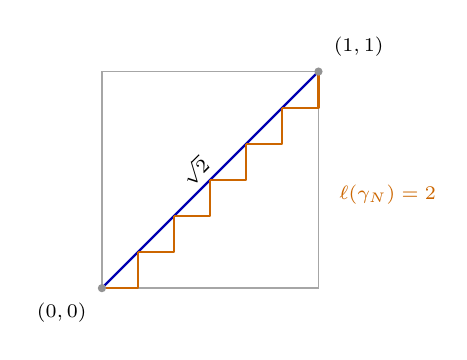
\begin{tikzpicture}[
  scale=2.75,
  every node/.style={font=\scriptsize},
  side/.style={gray!70, line width=0.55pt},
  chord/.style={blue!70!black, line width=0.85pt},
  stair/.style={orange!80!black, line width=0.8pt, line join=round},
  point/.style={circle, fill=gray!85, inner sep=1.05pt},
  labelbox/.style={fill=white, fill opacity=0.88, text opacity=1, inner sep=1.1pt}
]
  \coordinate (A) at (0,0);
  \coordinate (B) at (1,1);

  \draw[side] (0,0) rectangle (1,1);

  \draw[chord] (A) -- (B);

  \foreach \i in {0,...,5} {
    \draw[stair] ({\i/6},{\i/6}) -- ({(\i+1)/6},{\i/6}) -- ({(\i+1)/6},{(\i+1)/6});
  }

  \node[point] at (A) {};
  \node[point] at (B) {};
  \node[below left=2pt] at (A) {$(0,0)$};
  \node[above right=2pt] at (B) {$(1,1)$};

  \node[labelbox, rotate=45] at (0.43,0.54) {$\sqrt{2}$};
  \node[orange!80!black, labelbox, anchor=west] at (1.08,0.43) {$\ell(\gamma_N)=2$};
\end{tikzpicture}

  \caption{A staircase path can approach the diagonal in position while its polygonal length stays $2$, not $\sqrt{2}$.}
  \label{fig:staircase-length-vs-chord}
\end{figure}

\begin{perspective} \label{per:length-is-not-position-limit} \hlt{Length Is Not Just Shape}\\
Length is a supremum over partitions of one curve. Passing lengths through curve limits needs more than positional convergence; Theorem \ref{thm:continuously-differentiable-curves-rectifiable} uses $C^1$ speed control.
\end{perspective}

\begin{theorem} \label{thm:continuously-differentiable-curves-rectifiable} \hlt{Length of a Continuously Differentiable Curve}\\
If $\gamma':[a,b]\to\R^k$ is continuous, then $\gamma$ is rectifiable and $\ell(\gamma)=\int_a^b\norm{\gamma'(t)}\,dt$.
\begin{proof}
For $\Pi=\{x_0,\ldots,x_n\}$, Theorem \ref{thm:vector-valued-integral-results}(i) gives $\norm{\gamma(x_i)-\gamma(x_{i-1})} =\norm{\int_{x_{i-1}}^{x_i}\gamma'(t)\,dt} \leq\int_{x_{i-1}}^{x_i}\norm{\gamma'(t)}\,dt$.\\
Hence $\ell(\Pi,\gamma)\leq\int_a^b\norm{\gamma'}$. Conversely, choose $\Pi$ so fine that $\norm{\gamma'(s)-\gamma'(t)}<\varepsilon$ on each subinterval.\\
Choose $t_i\in[x_{i-1},x_i]$. Then $\int_{x_{i-1}}^{x_i}\norm{\gamma'(t)}\,dt \leq \norm{\gamma'(t_i)}\Delta x_i+\varepsilon\Delta x_i$.\\
Also $\gamma(x_i)-\gamma(x_{i-1})=\int_{x_{i-1}}^{x_i}\gamma'(t)\,dt$, so $\norm{\gamma'(t_i)}\Delta x_i \leq \norm{\gamma(x_i)-\gamma(x_{i-1})}+\varepsilon\Delta x_i$.\\
Thus $\int_{x_{i-1}}^{x_i}\norm{\gamma'(t)}\,dt \leq \norm{\gamma(x_i)-\gamma(x_{i-1})}+2\varepsilon\Delta x_i$.\\
Summing gives $\int_a^b\norm{\gamma'}\leq\ell(\gamma)+2\varepsilon(b-a)$; let $\varepsilon\downarrow0$.\\
\hlt{Structural Commentary}: Upper bounds are immediate; uniform continuity gives matching lower bounds.\\
\hlt{Key Insight}: For $C^1$ curves, length is accumulated speed.
\end{proof}
\end{theorem}

\begin{method} \label{meth:riemann-stieltjes-no-overlap-source-todo}\label{meth:riemann-stieltjes-proof-patterns} \hlt{Integration Proof Patterns}
\begin{enumerate}[label=(\roman*)]
\setlength{\itemsep}{0pt}
\item \hlt{Definitions}: fix $\Pi=\{x_i\}_{i=0}^n$ before defining $M_i,m_i,\Delta x_i,\Delta\alpha_i$.
\item \hlt{Refinement}: prove the one-point insertion case; iterate.
\item \hlt{Integrability}: find $\Pi$ with $U(\Pi,f,\alpha)-L(\Pi,f,\alpha)<\varepsilon$.
\item \hlt{Bad sets}: cover $E$ by $I_j=[u_j,v_j]$ with $\sum_j[\alpha(v_j)-\alpha(u_j)]<\varepsilon$; control $K=[a,b]\setminus\bigcup_j(u_j,v_j)$ uniformly.
\item \hlt{Properties}: pass to a common refinement before comparing sums.
\item \hlt{Calculus}: use the mean value theorem to form tagged sums, then apply Theorem \ref{thm:tagged-riemann-stieltjes-sums}.
\item \hlt{Improper integrals}: truncate endpoints; use monotonicity or tail bounds.
\end{enumerate}
\hlt{Key Insight}: Riemann--Stieltjes integration is Darboux approximation plus a choice of interval weights $\Delta\alpha_i$.
\end{method}
